\chapter{Mechanical Systems}

\section{Introduction}
The Mechanical Department of the Hyperloop team is crucial for the design, development, and implementation of the mechanical systems within the Hyperloop pod. This department focuses on creating innovative solutions to achieve optimal performance, safety, and reliability in the pod's operation. It is responsible for the design and engineering of key mechanical components, including the chassis, suspension, braking systems, and aerodynamics.\\
\\
Chassis: This subdepartment is responsible for designing the pod's leightweight frame or skeleton. The chassis is the foundation that supports all other mechanical components, ensuring they work in harmony. It's engineered to be robust yet lightweight, balancing structural integrity with performance efficiency.

Suspension: The suspension team focuses on the system that connects the chassis to the tracks, absorbing vibrations and shocks to maintain stability during high-speed travel. Their work is crucial for the pod's handling and ride quality.

Braking: Essential for safety and control, the braking subdepartment designs systems to decelerate the pod efficiently. This involves selecting materials and mechanisms that ensure reliable and effective stopping power, considering the pod's high-speed nature.

Aerodynamics: This group works on optimizing the pod's shape and surface to minimize air resistance, which is vital for achieving high speeds and efficient energy use. Their work includes designing the pod's external shell and analyzing airflow to enhance performance.\\
\\
Each subdepartment plays a critical role in the pod's overall design and function, working together to tackle the unique challenges of Hyperloop technology. Their collaborative efforts ensure the pod is safe, efficient, and ready to redefine high-speed transportation.


\section{Chassis}




\subsection{Overview}


\subsubsection{Requirements and Constraints}

Paramount among our requirements is the ability of the chassis to withstand the rigors of operation, with a primary focus on supporting a load of up to 250 kg. The chassis must serve as the sturdy foundation upon which all subsystems are mounted. From the propulsion system to the suspension components, every subsystem must find its place within the chassis. 

A chassis that is inaccessible is as good as useless. Hence, a key requirement driving our design is the ease of access for maintenance and assembly. Components must be readily accessible, allowing for swift troubleshooting and efficient assembly processes. The chassis must seamlessly integrate with the aeroshell, providing a secure mounting point while ensuring aerodynamic efficiency. This requirement necessitates careful consideration of mounting points and structural reinforcements to support the aeroshell without compromising performance. 

Weight is the enemy of performance, and our chassis must strike a delicate balance between structural robustness and lightweight construction. Utilizing advanced materials and optimization techniques, we aim to minimize weight without compromising strength or durability. 

While performance is paramount, cost considerations cannot be overlooked. Our chassis must be constructed in a manner that balances performance with affordability, ensuring that our project remains economically viable without sacrificing quality or functionality. The chassis must withstand the dynamic forces exerted by both the braking system and the suspension components. 

This constraint necessitates careful reinforcement and structural design to ensure that the chassis remains resilient under varying load conditions. The design must incorporate provisions for easy extraction of the battery pack, facilitated by a rail system. This constraint imposes additional design considerations, such as clearance and mounting points, to ensure seamless integration and accessibility.


\subsubsection{Concept}

The chassis plays an important role in any moving structure, providing the structural foundation and support necessary to ensure safety, stability, and functionality for the entire vehicle and all the systems it holds. 
In this year's iteration, our pod utilises a two-track system, which not only allows for extra room to house subsystems but also lowers the pod's centre of mass, thereby enhancing stability. This design decision results in a wider and consequently shorter pod.

At the core of our design philosophy lies the integration of carbon fiber sandwich plates, a cutting-edge material renowned for its exceptional strength-to-weight ratio and structural integrity.
The foundation of our chassis is built upon a rectangular framework, strategically crafted to optimize both stability and versatility. Covering the entirety of the lower section of the pod is a ground plate, providing a robust foundation while simultaneously enhancing aerodynamic efficiency. This ground plate serves as the backbone of the chassis, ensuring unparalleled stability and structural integrity.

Extending longitudinally from the front to the back of the pod are two key components: the longitudinal plates. These plates constitute the primary structural elements of the chassis, serving as the anchor points for vital components such as the suspension system, brakes, and motor. Crafted with precision and reinforced for maximum resilience, these longitudinal plates epitomize the marriage of form and function, providing the framework upon which our pod's performance hinges.

To further fortify the structural integrity of our chassis and prevent any potential bending or detachment of the longitudinal plates, we have strategically incorporated three additional cross panels. These panels, positioned perpendicular to the longitudinal plates, serve as stabilizing agents, distributing forces evenly throughout the chassis and bolstering overall rigidity. these cross panels ensure that our pod remains steadfast and unwavering, even under the most demanding conditions.

Central to the assembly of our chassis is a plug-in system, integrated into the carbon fiber sandwich plates. Through precision-cut cutouts and advanced adhesive technologies, these plates seamlessly interlock and adhere, forming a cohesive and resilient structure. This plug-in system not only streamlines the assembly process but also enhances the overall integrity of the chassis, ensuring a robust and reliable foundation for our pod.


\subsubsection{Size, Components, and Appearance}

\begin{table}[ht]
\centering

\label{table:components}
\begin{adjustbox}{width=\textwidth,center}
\begin{tabular}{|>{\bfseries}m{2.5cm}|m{1.4cm}|m{1.7cm}|m{2.1cm}|m{2.2cm}|m{2.6cm}|m{2.2cm}|}
\hline
Component & Number & Mass [kg] & Size [mm] & Material & Manufacturing process & In-house/ outsourced \\
\hline
GP & x1 & 1 & 1480x882x20 & CF Sandwich & Waterjetcut & Outsourced \\
CacP & x1 & 1 & 882x200x20 & CF Sandwich & Waterjetcut & Outsourced \\
BacP & x2 & 0.1 & 882x200x20 & CF Sandwich & Waterjetcut & Outsourced \\
BCalP & x2 & 0.2 & 883x200x20 & CF Sandwich & Waterjetcut & Outsourced \\
AalP & x2 & 0.2 & 270x200x20 & CF Sandwich & Waterjetcut & Outsourced \\
Seam Type A & x2 & 0.1 & 1480x882x1 & CF Prepeg & Cut & Outsourced \\
Seam Type B & x7 & 0.1 & 882x200x1 & CF Prepeg & Cut & Outsourced \\
Seam Type C & x2 & 0.1 & 882x200x1 & CF Prepeg & Cut & Outsourced \\
Seam Type D & x2 & 0.1 & 883x200x1 & CF Prepeg & Cut & Outsourced \\
Crossbar & x2 & 0.5 & 270x200x20 & Aluminium & Waterjetcut & Outsourced \\
\hline

\end{tabular}
\end{adjustbox}
\caption{Components and Manufacturing Details}
\end{table}




\subsection{Theoretical concepts}

\textbf{WILL BE ADDED SOON}




\subsection{Design Process and Appearance}


\subsubsection{CAD Models and Technical Drawings}

%\begin{comment}
\begin{figure}[ht]
  \centering
  
\includegraphics[width=\linewidth]{texfiles/mech/updated/chassis/cad1.png}
  \caption{Caption for the image.}
  \label{fig:image1}
\end{figure}

\begin{figure}[ht]
  \centering
  \subfloat[Caption for the first image.]{
    \centering
    \includegraphics[width=0.5\linewidth]{texfiles/mech/updated/chassis/technicaldrawing1.png}
    \label{fig:sub1}
  }
  \subfloat[Caption for the second image.]{
    \centering
    \includegraphics[width=0.5\linewidth]{texfiles/mech/updated/chassis/technicaldrawing1.png}
    \label{fig:sub2}
  }
  \caption{Caption for the whole figure.}
  \label{fig:test}
\end{figure}

\begin{figure}[ht]
  \centering
  \subfloat[Caption for the first image.]{
    \centering
    \includegraphics[width=0.5\linewidth]{texfiles/mech/updated/chassis/technicaldrawing1.png}
    \label{fig:sub1}
  }
  \subfloat[Caption for the second image.]{
    \centering
    \includegraphics[width=0.5\linewidth]{texfiles/mech/updated/chassis/technicaldrawing1.png}
    \label{fig:sub2}
  }
  \caption{Caption for the whole figure.}
  \label{fig:test}
\end{figure}

%\end{comment}


\subsubsection{Materials}

As discribed above the main factor for choosing carbon fiber sandwich panels was the the weight-strenght-cost balance. Choosing a foam-insert over a honeycomb-insert came down to the higher weather-resistants of the foam against cardboard. Again we chose carbonfiber over aluminum for the plates for lesser weight.


\subsubsection{Design Rationale}

The design rationale guiding our pod's infrastructure embodies a methodical process rooted in practical considerations and engineering principles. Our primary aim was to reduce weight from the previous design, leading us to explore the potential of carbon fiber composites.

Initially, a monocoque chassis was considered for its structural integrity, yet its high cost and manufacturing complexity deemed it impractical. Similarly, the idea of a tube chassis with carbon fiber tubes proved prohibitively expensive. Thus, we opted for a Composite Sandwich Panel Chassis, renowned for its lightweight, structural strength, and cost-effectiveness. 

Departing from the original design, which featured longitudinal panels spanning the entire length of the pod, we recognized the necessity for easy battery extraction from the side, prompting a redesign of the chassis layout. To ensure seamless panel interlocking and structural integrity, we devised a plug-in system featuring evenly distributed cutouts, meticulously aligned for connection. These connections are strengthened by precise gluing and reinforced seaming along the edges.

Additionally, crossbars were strategically integrated to fortify the chassis at suspension mounting points, mitigating potential structural weaknesses. Furthermore, close collaboration between the chassis department and other subsystems facilitated maximal compatibility and integration.

In summary, our design rationale represents a pragmatic synthesis of innovation and engineering expertise, driven by a commitment to efficiency, functionality, and cost-effectiveness.


\subsubsection{FEM Results}

\paragraph{Static Simulation Stress Test:}
In this simulation scenario, the chassis was subjected to a static stress test, replicating the forces exerted by the suspension system along with the weight of the pod. The FEM analysis yielded critical insights into the structural performance of the chassis under static loading conditions.

\paragraph{Results:}
\begin{itemize}
    \item\textbf{Maximum von Mises stress:} [Replace with your FEM result]
    \item\textbf{Maximum principal stress:} [Replace with your FEM result]
    \item\textbf{Factor of safety:} [Replace with your FEM result]
\end{itemize}

\paragraph{Interpretation: }
The FEM analysis indicates that under static loading conditions, the chassis exhibits [Replace with your interpretation of FEM results]. While localized areas may experience elevated stress levels, the overall factor of safety remains within acceptable limits, suggesting satisfactory structural integrity.

\paragraph{Braking Maneuver Simulation}
In this simulation scenario, the chassis underwent analysis with peak forces experienced during braking maneuvers, simulating the most demanding braking conditions. The FEM analysis provided crucial insights into the chassis's ability to withstand dynamic braking forces.

\paragraph{Results:}
\begin{itemize}
    \item\textbf{Maximum von Mises stress:} [Replace with your FEM result]
    \item\textbf{Maximum principal stress:} [Replace with your FEM result]
    \item\textbf{Factor of safety:} [Replace with your FEM result]
\end{itemize}

\paragraph{Interpretation: }
The FEM analysis reveals that during braking maneuvers, the chassis experiences [Replace with your interpretation of FEM results]. Despite localized stress concentrations, the overall factor of safety remains satisfactory, indicating adequate structural robustness.

\paragraph{Worst-Case Scenario:}
In the worst-case scenario simulation, the chassis was subjected to double the forces encountered in the previous scenarios, representing an extreme operating condition. This simulation aimed to assess the chassis's resilience under significantly elevated loading conditions.

\paragraph{Results:}
\begin{itemize}
    \item\textbf{Maximum von Mises stress:} [Replace with your FEM result]
    \item\textbf{Maximum principal stress:} [Replace with your FEM result]
    \item\textbf{Factor of safety:} [Replace with your FEM result]
\end{itemize}

\paragraph{Interpretation: }
The FEM analysis of the worst-case scenario indicates [Replace with your interpretation of FEM results]. Despite heightened stress levels, the factor of safety remains within acceptable limits, suggesting that the chassis can withstand double the expected forces without compromising structural integrity.

\paragraph{Conclusion:}
Overall, the FEM results provide valuable insights into the structural performance of the chassis under various loading conditions. These findings will inform further optimization efforts and ensure that the chassis meets stringent performance and reliability requirements.

%\begin{comment}
\begin{figure}[ht]
  \centering
  \includegraphics[width=\linewidth]{texfiles/mech/updated/chassis/fem1.png}
  \caption{Caption for the image.}
  \label{fig:image1}
\end{figure}

\begin{figure}[ht]
  \centering
  \subfloat[Caption for the first image.]{
    \centering
    \includegraphics[width=0.5\linewidth]{texfiles/mech/updated/chassis/fem1.png}
    \label{fig:sub1}
  }
  \subfloat[Caption for the second image.]{
    \centering
    \includegraphics[width=0.5\linewidth]{texfiles/mech/updated/chassis/fem1.png}
    \label{fig:sub2}
  }
  \caption{Caption for the whole figure.}
  \label{fig:test}
\end{figure}


\subsubsection{Calculations}

In order to ensure the accuracy and reliability of the Finite Element Method (FEM) simulations, it is crucial to provide a comprehensive justification for the simulated loads. The following reasoning and calculations support the chosen loads for each simulation scenario:

\begin{itemize}
  \item \textbf{Static Simulation Stress Test}
    \begin{itemize}
      \item \textbf{Reasoning:} The static simulation stress test replicates the forces exerted by the 		suspension system and the weight of the pod when the vehicle is at rest or moving at a 					constant velocity. This scenario is essential to evaluate the chassis's ability to withstand 				static loading conditions, providing insights into its structural integrity and load-bearing 				capacity.

	  \item \textbf{1.	Suspension Forces:} 
		The suspension system applies forces to the chassis, primarily in the vertical direction, to 				support the weight of the vehicle and absorb road irregularities.

	  \item \textbf{Average Suspension Force (Fsus):}
		(Insert calculation based on suspension design and vehicle weight distribution)

	  \item \textbf{2.	Weight of the Pod:} 
		The weight of the pod contributes to the overall static loading on the chassis.

	  \item \textbf{Pod Weight (Wpod):} 
		(Insert actual weight of the pod)

	  \item \textbf{Total Load:}
		Total Load = Suspension Forces + Weight of the Pod Total Load = Fsus + Wpod
	\end{itemize}
\end{itemize}

\begin{itemize}
  \item \textbf{Braking Maneuver Simulation}
    \begin{itemize}
      \item \textbf{Reasoning:} The braking maneuver simulation replicates the peak forces experienced 		by the chassis during braking events. This scenario is crucial to assess the chassis's ability 		to withstand dynamic loading conditions, particularly during sudden deceleration, and ensure 				structural stability and safety.

	  \item \textbf{1.	Peak Braking Force:} 
		The braking system applies forces to the chassis during braking maneuvers, primarily in the 				longitudinal direction, to decelerate the vehicle.

	  \item \textbf{Peak Braking Force (Fbrake):}
		(Insert calculation based on braking system specifications and vehicle weight)
	\end{itemize}
\end{itemize}
	
\begin{itemize}  
  \item \textbf{Worst-Case Scenario:}
	\begin{itemize}
	  \item \textbf{Reasoning:} The worst-case scenario involves doubling the forces encountered in 				the previous scenarios, representing an extreme operating condition. This scenario tests the 				limits of the chassis's structural resilience and provides insights into its performance under 		significantly elevated loading 
		conditions.

	  \item \textbf{1.	Double Suspension Forces:} The suspension forces are doubled to simulate 					extreme vertical loading conditions on the chassis.
-	Double Suspension Forces (2 * Fsus)

	  \item \textbf{1.	Double Braking Forces:}The braking forces are doubled to simulate extreme 				braking maneuvers.
-	Double Braking Forces (2 * Fbrake)

	  \item \textbf{Conclusion:} By providing rigorous justification and performing the necessary load 		calculations, we ensure that the simulated loads accurately represent real-world operating 				conditions. These simulations enable us to evaluate the structural performance of the chassis 				under various loading scenarios, guiding optimization efforts and ensuring the chassis meets 				stringent performance requirements.

	\end{itemize}
\end{itemize}


-	Acceleration due to gravity: \(9.81\frac{m}{s^2}\)
-	Weight of the pod (W\_pod) = Mass of the pod × Acceleration due to gravity

2.	Forces from Suspension:
-	Suspension force: [Replace with actual suspension force]
-	Total force from suspension (F\_suspension) = Suspension force × Number of suspension points

3.	Total Static Load:
-	Total static load = Weight of the pod + Total force from suspension

Simulation Scenario 2: Braking Maneuver Simulation

1.	Peak Braking Force:
-	Maximum deceleration: [Replace with actual maximum deceleration]
-	Mass of the vehicle: [Replace with actual mass]
-	Peak braking force = Mass of the vehicle × Maximum deceleration

Worst-Case Scenario:

1.	Double Forces:
-	Double weight of the pod: 2 × Weight of the pod
-	Double total


\subsubsection{Mesh and Boundary Conditions}

Mesh Type: For our Finite Element Method (FEM) simulations, we utilized a structured mesh approach, specifically employing a combination of hexahedral and tetrahedral elements. This mesh type offers several advantages, including improved computational efficiency, better accuracy in capturing complex geometries, and reduced numerical error.

Boundary Conditions:

1.	Fixed Constraints:
-	Suspension Mounting Points: The chassis is fixed at the suspension mounting points to simulate the rigid attachment of the suspension system to the chassis.
-	Ground Contact: The bottom surface of the chassis is fixed to simulate contact with the ground, ensuring realistic loading conditions.

2.	Applied Loads:
-	Suspension Forces: Vertical forces are applied at the suspension mounting points to simulate the forces exerted by the suspension system on the chassis. These forces represent the weight of the vehicle and any additional loads imposed by the suspension system.
-	Braking Forces: Longitudinal forces are applied to simulate the braking forces exerted on the chassis during braking maneuvers. These forces are applied at the contact points between the braking system and the chassis.

3.	Symmetry and Constraints:
-	Symmetry: Symmetry boundary conditions are applied to exploit the symmetry of the chassis geometry, reducing computational complexity and improving efficiency.
-	Constraints: Constraints are imposed on certain degrees of freedom to enforce realistic behavior and prevent unrealistic deformations or displacements.

4.	Mesh Refinement:
-	Local Mesh Refinement: Mesh refinement techniques are applied in areas of geometric complexity or high stress concentration to ensure accurate representation of stress distribution and structural response.

Conclusion: By employing a structured mesh approach and carefully defining boundary conditions, we ensure that our FEM simulations accurately capture the behavior of the chassis under various loading scenarios. These simulations provide valuable insights into the structural performance of the chassis, guiding optimization efforts and ensuring that the design meets stringent performance requirements.

\textbf{WILL BE ADDED SOON}

\begin{comment}
\begin{figure}[ht]
  \centering
  \subfloat[Caption for the first image.]{
    \centering
    \includegraphics[width=0.5\linewidth]{texfiles/mech/updated/chassis/mesh1.png}
    \label{fig:sub1}
  }
  \subfloat[Caption for the second image.]{
    \centering
    \includegraphics[width=0.5\linewidth]{texfiles/mech/updated/chassis/mesh1.png}
    \label{fig:sub2}
  }
  \caption{Caption for the whole figure.}
  \label{fig:test}
\end{figure}
\end{comment}




\subsection{Manufacturing Process}

Firstly, the panels are sourced and procured in accordance with precise specifications, ensuring they meet the required size and shape criteria. Any necessary cutouts or holes are meticulously made in alignment with design specifications, utilizing advanced cutting techniques to ensure accuracy and consistency. Subsequently, support plates are precisely cut to the required size and shape, with corresponding holes carefully drilled to facilitate seamless integration with the panels. 

These support plates serve a critical role in reinforcing the structural integrity of the chassis, providing additional strength and stability. Following preparation of the panels and support plates, a meticulous assembly process ensues. The support plates are methodically glued to the designated spots on the panels, adhering to precise positioning guidelines to ensure optimal alignment and functionality.

Once the support plates are securely affixed, the panels are carefully assembled and glued together, forming a cohesive structure that embodies the desired design configuration. This assembly process is executed with meticulous attention to detail, ensuring that each component is seamlessly integrated to achieve the desired structural integrity and functionality.

Finally, the seams between the assembled panels are meticulously cut to the required size and adhered to the edges of the plugged panels. This final step serves to further reinforce the structural integrity of the chassis while providing a polished finish that enhances both aesthetics and durability. Through adherence to this comprehensive manufacturing process, we ensure that the designed part is not only realized in a practical and efficient manner but also upholds the highest standards of quality and performance.

\textbf{or:}

Efforts have been undertaken to ensure that the designed part is realistically manufacturable, with a focus on simplicity, efficiency, and accessibility in manufacturing processes.

1.	2D Waterjet Cutting for Panels: Utilizing 2D waterjet cutting for the panels ensures precise and efficient fabrication. This method allows for accurate cutting of complex shapes and contours, facilitating the production of panels with minimal material wastage.

2.	Scissor-Cut Seams: Seam cutting by scissors offers a straightforward and cost-effective approach to joining panels. This manual method provides flexibility and ease of assembly, allowing for adjustments as needed during the manufacturing process. Additionally, it eliminates the need for specialized equipment, reducing production costs and complexity.

3.	Waterjet Cutting for Plates: Employing waterjet cutting for the plates ensures accurate and clean cuts, maintaining dimensional accuracy and quality. This method allows for the fabrication of support plates with intricate designs and precise hole placements, enabling optimal integration with the chassis components.

By leveraging these manufacturing techniques, we streamline the production process while maintaining the integrity and functionality of the designed part. The simplicity and accessibility of these methods ensure that the manufacturing process remains efficient, cost-effective, and scalable, ultimately contributing to the overall success of the project.




\subsection{Integration process}


\subsubsection{Assembling}

Firstly, the panels are sourced and procured in accordance with precise specifications, ensuring they meet the required size and shape criteria. Any necessary cutouts or holes are meticulously made in alignment with design specifications, utilizing advanced cutting techniques to ensure accuracy and consistency.

Subsequently, support plates are precisely cut to the required size and shape, with corresponding holes carefully drilled to facilitate seamless integration with the panels. These support plates serve a critical role in reinforcing the structural integrity of the chassis, providing additional strength and stability.

Following preparation of the panels and support plates, a meticulous assembly process ensues. The support plates are methodically glued to the designated spots on the panels, adhering to precise positioning guidelines to ensure optimal alignment and functionality.

Once the support plates are securely affixed, the panels are carefully assembled and glued together, forming a cohesive structure that embodies the desired design configuration. This assembly process is executed with meticulous attention to detail, ensuring that each component is seamlessly integrated to achieve the desired structural integrity and functionality.

Finally, the seams between the assembled panels are meticulously cut to the required size and adhered to the edges of the plugged panels. This final step serves to further reinforce the structural integrity of the chassis while providing a polished finish that enhances both aesthetics and durability.

Through adherence to this comprehensive manufacturing process, we ensure that the designed part is not only realized in a practical and efficient manner but also upholds the highest standards of quality and performance.

\subsubsection{Assembly interaction}


The interaction between subsystems within the pod is orchestrated with precision, each component playing a crucial role in ensuring seamless functionality and performance. At the heart of this interaction lies the chassis, serving as the sturdy backbone upon which all subsystems are mounted. The chassis not only provides structural support but also serves as a conduit for distributing forces generated by key subsystems such as the brakes, motor, and suspension.

The motor, positioned centrally within the pod, exerts significant forces that are channeled directly through the chassis. As the primary source of propulsion, the motor's torque and power output directly influence the chassis's stability and performance. Similarly, the braking system, situated on the sides directly above the track, exerts substantial forces during deceleration. These forces are transmitted through the chassis, requiring robust structural reinforcement to withstand the resulting stresses.

The suspension system, located at the front and back ends of the pod, plays a critical role in ensuring ride comfort and handling. The forces generated by the suspension, particularly during cornering and uneven terrain traversal, are transmitted through the chassis, necessitating careful design considerations to maintain stability and responsiveness.

In addition to these dynamic subsystems, the electrical systems are integrated into the chassis using sheet metal and 3D-printed brackets. This strategic mounting ensures secure placement while minimizing interference with other components.

Furthermore, the battery, housed within a dedicated battery box, is mounted on telescopic rails affixed to the chassis. This arrangement not only facilitates easy access for maintenance but also ensures optimal weight distribution and stability.

Through integration and strategic mounting, each subsystem interacts harmoniously with the chassis and other components, collectively contributing to the overall functionality and performance of our pod. This cohesive interaction is essential for achieving our objectives of efficiency, reliability, and safety.




\subsection{Safety Considerations}


\subsubsection{Safety Factor}

For our project, we have established a minimum safety factor of n=2 for all structural elements. This means that the ultimate strength of each component must be at least twice the maximum expected load it will experience.

Reaching a safety factor of n=… provides a significant margin of safety, offering protection against unforeseen variations in loading conditions, material properties, and environmental factors. It ensures that the structural elements can withstand unexpected peak loads or transient events without compromising safety or integrity.


\subsubsection{Worst-Case Scenarios}

\textbf{WILL BE ADDED SOON}




\subsection{FMEA Results Discussion}


\subsubsection{Risk Assessment}

\textbf{WILL BE ADDED SOON}


\subsubsection{FMEA and Risk Mitigation}
\begin{comment}
\textbf{WILL BE ADDED SOON}
\begin{figure}[ht]
  \centering
  
\includegraphics[width=\linewidth]{texfiles/mech/updated/chassis/FMEA1.png}
  \caption{Caption for the image.}
  \label{fig:image1}
\end{figure}
\end{comment}

\subsubsection{Simulation Evidence}

\textbf{WILL BE ADDED SOON}




\subsection{Testing}


\subsubsection{Safety Procedures Documentation}

The testing procedures for the hyperloop pod chassis are meticulously crafted to assess structural integrity, durability, and performance under conditions that closely simulate actual operation. The procedures outlined below provide a comprehensive approach to validating the chassis design.

\paragraph{Static Load Testing}
\begin{itemize}
    \item \textbf{Objective:} To evaluate the chassis's ability to withstand forces it would encounter while stationary.
    \item \textbf{Procedure:} Securely mount the chassis at suspension mounting holes. Apply a static load equivalent to twice the anticipated weight of the finished pod.
    \item \textbf{Outcome:} Determine load-bearing capacity and ensure no structural deformation or failure.
\end{itemize}

\paragraph{Dynamic Load Testing}
\begin{itemize}
    \item \textbf{Objective:} To assess the chassis's responsiveness and robustness under dynamic loading conditions.
    \item \textbf{Procedure:} Subject the chassis to simulated forces of acceleration, braking, and cornering. Collect data on how the chassis flexes and reacts under these conditions.
    \item \textbf{Outcome:} Confirm the chassis's integrity under dynamic stresses and identify potential areas for reinforcement.
\end{itemize}

\paragraph{Bending Stress Test}
\begin{itemize}
    \item \textbf{Objective:} To understand the material properties of the chassis, particularly its bending strength and ductility.
    \item \textbf{Procedure:} Fabricate a reference part from the same material as the chassis. Apply incremental force until the part fails, if applicable.
    \item \textbf{Outcome:} Ascertain the material's resistance to bending forces and its behavior under stress.
\end{itemize}

\paragraph{Vibration Testing}
\begin{itemize}
    \item \textbf{Objective:} To evaluate the chassis's ability to endure and dampen vibrations during operation.
    \item \textbf{Procedure:} Expose the chassis to controlled vibrations at various frequencies and amplitudes to simulate motor-generated vibrations and other operational scenarios.
    \item \textbf{Outcome:} Ensure the chassis can effectively dampen vibrations and avoid resonance or structural fatigue.
\end{itemize}


\subsubsection{preliminary testing plan}

This section outlines the testing plan for the chassis of the hyperloop pod, ensuring its structural integrity and stability under various loads and conditions.

\paragraph{Static Load Testing}
\begin{itemize}
    \item \textbf{Method:} Securely mount the chassis at the suspension mounting holes.
    \item \textbf{Loading:} Apply a static load equivalent to twice the weight of the finished pod.
    \item \textbf{Duration:} Maintain the load for a predetermined period to assess the structural integrity.
    \item \textbf{Measurement:} Monitor for deformation or failure.
\end{itemize}

\paragraph{Dynamic Load Testing}
\begin{itemize}
    \item \textbf{Method:} Simulate dynamic forces experienced during operation.
    \item \textbf{Loading:} Apply forces to replicate acceleration, braking, and cornering.
    \item \textbf{Duration:} Perform over various speeds and conditions.
    \item \textbf{Measurement:} Record deflection and structural response.
\end{itemize}

\paragraph{Bending Stress Test}
\begin{itemize}
    \item \textbf{Method:} Use a reference part made from the same material as the chassis panels.
    \item \textbf{Loading:} Incrementally apply force until failure.
    \item \textbf{Measurement:} Note the force applied and deformation at failure.
    \item \textbf{Expected Result:} Determine material's bending strength and ductility.
\end{itemize}

\paragraph{Vibration Testing}
\begin{itemize}
    \item \textbf{Method:} Subject chassis to controlled vibrations across frequencies.
    \item \textbf{Loading:} Simulate operational vibrations.
    \item \textbf{Duration:} Extend testing for durability assessment.
    \item \textbf{Measurement:} Assess chassis damping and response to vibrations.
    \item \textbf{Expected Result:} Ensure chassis can maintain integrity under vibration.
\end{itemize}

\paragraph{Expected Results}
The chassis is expected to demonstrate stability and maintain structural integrity under static and dynamic loads. The bending stress test will confirm the material's properties, while vibration testing will validate damping capabilities. Through this comprehensive testing, the chassis will be proven to meet rigorous quality and safety standards, crucial for the hyperloop pod's performance.



\section{Suspension}

\subsection{Introduction}
\subsubsection{Overview of the System}
The front and rear double wishbone suspension system serves as a critical component within our Hyperloop pod, aimed at delivering a comfortable and stable ride experience. At its core lies the circular knuckle, meticulously designed to accommodate essential parts like bearings, retaining rings, and shafts. This central hub enables smooth vertical movement of the suspension, absorbing track imperfections for a seamless ride. Wishbones attached to the knuckle control suspension motion, featuring specialized bearings to maintain precise alignment. Dampeners directly connected to the knuckle assembly absorb shocks and vibrations, enhancing responsiveness to terrain changes. Additionally, a linkage mechanism minimizes lateral movement, ensuring stability, especially during high-speed travel. Integration with the chassis is facilitated by high-performance bearings, allowing for articulation and load transfer.

\subsubsection{Requirements and Constraints}
The suspension system must meet stringent requirements to ensure optimal performance and safety. It must provide exceptional ride quality, stability, and control throughout the journey, from acceleration to high-speed cruising. Constraints include optimizing weight distribution and reducing unsprung mass to enhance handling dynamics. The system must also minimize lateral sway and maintain course stability under demanding conditions. Incorporation of specialized bearings like the Female Wiebel Bearing further enhances stability and control. Meticulous engineering is essential to meet these requirements while adhering to space, weight, and durability constraints inherent to Hyperloop pod design.

\newpage
\subsection{Subsystem Overview}
\subsubsection{Explanation of Subsystem Concepts}
\textbf{Control Arms:} The control arms are the primary components of the double wishbone suspension system, forming the distinctive "double wishbone" shape. These arms connect the Knuckle to the vehicle's chassis, with one arm positioned above and another below the wheel. They work together to control the wheel's vertical movement and maintain stability. This configuration allows the control arms to absorb bumps and shocks from the road while providing precise control over the wheel's motion.

\textbf{Shock Absorbers (Dampers):} Shock absorbers control the rate of compression and expansion of the springs, damping the oscillations of the suspension system caused by road imperfections. Shock absorbers play a crucial role in enhancing stability, comfort, and control by minimizing bounce and sway.

\newpage
\subsection{Theoretical Concepts}
\subsubsection{Detailed Explanation of Theoretical and Physical Principles}
\textbf{Theoretical Principles:}

\begin{enumerate}
    \item \textbf{Independent Suspension:}
    
    A fundamental theoretical principle underlying the double wishbone suspension is the provision of independent movement for each wheel. By decoupling the motion of one wheel from the other, this system ensures that disturbances affecting one wheel do not directly impact the other. This independence is crucial for maintaining optimal traction, stability, and comfort, particularly when navigating uneven terrain or cornering at high speeds. With independent suspension, variations in road surface or cornering forces can be effectively managed, enhancing overall vehicle dynamics.
    
\item \textbf{Controlled Wheel Movement:}
    
    The design of the wishbone-shaped control arms serves to control the movement of the wheel in multiple directions. These arms dictate the wheel's motion both vertically, for absorbing bumps and shocks, and horizontally, for steering input and stability. By strategically positioning and shaping the control arms, engineers can tailor the suspension's response to different driving conditions, ensuring precise handling and ride quality. This controlled movement allows for optimized wheel alignment, minimizing tire wear and maximizing grip, leading to improved overall performance and safety.
\end{enumerate}

\textbf{Physical Principles:}

\begin{enumerate}
    \item \textbf{Shock Absorption:}
    
    Shock absorption is a primary physical principle at work in a double wishbone suspension system. When the wheel encounters bumps or irregularities on the road surface, the suspension compresses and decompresses to absorb the impact. This process involves the coordinated action of the control arms and the shock absorbers (typically coilover or strut-type). The control arms guide the wheel's vertical movement, while the shock absorbers dampen the oscillations generated by road disturbances. Together, they mitigate the transmission of vibrations and shocks to the vehicle's chassis, providing occupants with a smoother and more comfortable ride experience.
    
    \item \textbf{Load Distribution and Handling:}
    
    Load distribution and handling are essential physical principles influenced by the double wishbone suspension design. By distributing the vehicle's weight more evenly across all four wheels, this suspension system enhances traction and stability, especially during acceleration, braking, and cornering maneuvers. The geometry of the control arms plays a critical role in determining the vehicle's handling characteristics. Optimal geometry helps manage weight transfer during dynamic driving situations, ensuring responsive steering, minimal body roll, and enhanced cornering ability. Additionally, the precise control over wheel movement provided by the double wishbone setup contributes to predictable and balanced handling, promoting driver confidence and safety on the road.
\end{enumerate}

\newpage
\subsubsection{Use of Free Body Diagrams for Load Cases}
\begin{figure}[ht!]
  \centering
  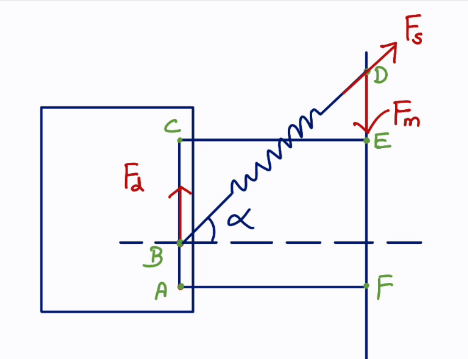
\includegraphics[width=\linewidth]{texfiles/mech/eimg/suspension/fbd.png}
  \caption{Caption for the image.}
  \label{fig:image1}
\end{figure}

\newpage
\begin{align*}
1. & \text{ Fs:} & \text{Force of Shock Absorber} \\
2. & \text{ Fd:} & \text{Force due to disturbances} \\
3. & \text{ Fm:} & \text{Force to weight of the Chassis} \\
4. & \alpha: & \text{Horizontal angle of the Shock Absorber} \\
5. & \text{ CE:} & \text{Upper Wishbone} \\
6. & \text{ AF:} & \text{Lower wishbone} \\
7. & \text{ AC:} & \text{Knuckle} \\
\end{align*}

\subsection{Design Process and Appearance}
\subsubsection{Presentation of CAD Models and Technical Drawings}
\begin{figure}[ht!]
  \centering
  \begin{subfigure}{.5\textwidth}
    \centering
    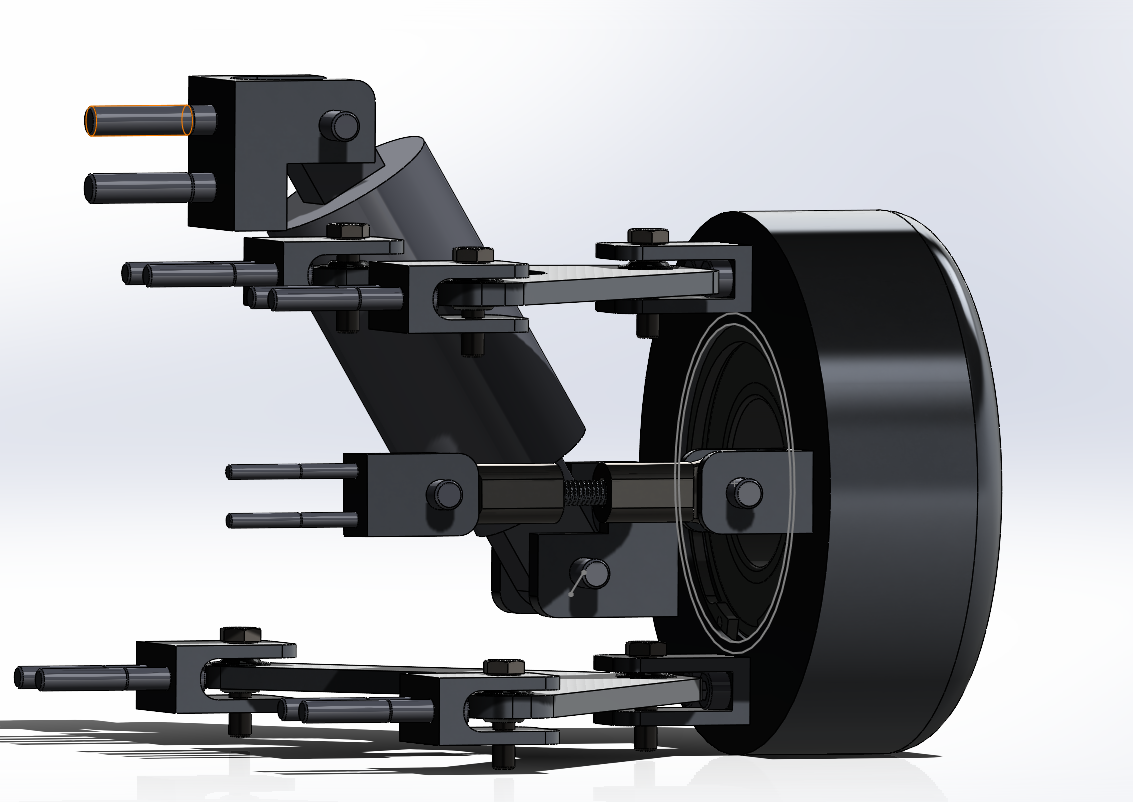
\includegraphics[width=\linewidth]{texfiles/mech/eimg/suspension/CAD_Deign of Rear Suspension.png}
    \caption{Caption for the first image.}
    \label{fig:sub1}
  \end{subfigure}%
  \begin{subfigure}{.5\textwidth}
    \centering
    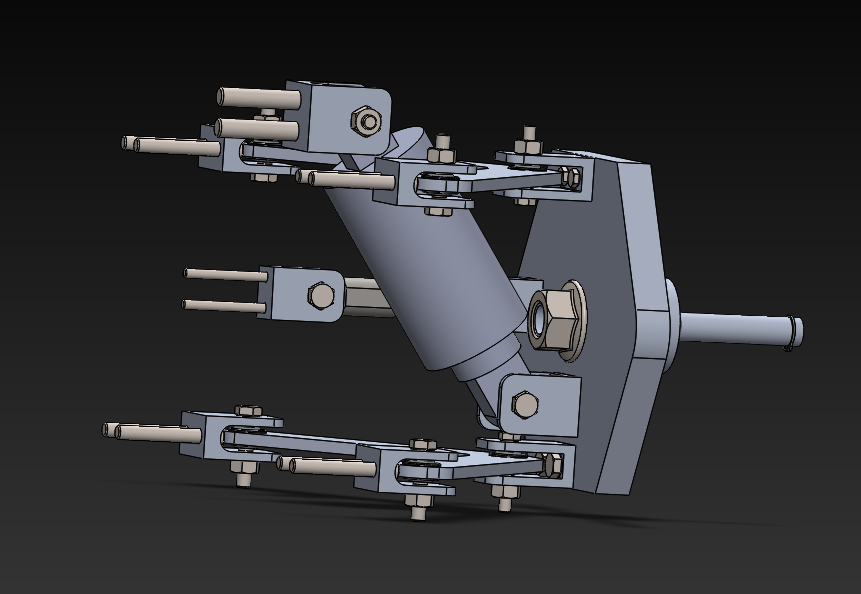
\includegraphics[width=\linewidth]{texfiles/mech/eimg/suspension/CAD Design Front wishbone Assembly.png}
    \caption{Caption for the second image.}
    \label{fig:sub2}
  \end{subfigure}%
\end{figure}
\newpage
\subsubsection{Justification of Material Selection}

\begin{itemize}
    \item \textbf{High Strength-to-Weight Ratio:} Utilizing Alloy 6061 would help reduce the overall weight of your suspension components while maintaining the necessary strength. This can improve the performance of your vehicle by reducing unsprung mass, which enhances handling, responsiveness, and fuel efficiency.
    
    \item \textbf{Corrosion Resistance:} The corrosion resistance of Alloy 6061 ensures the longevity and durability of your suspension components, especially considering the exposure to various environmental conditions and road debris that they may experience.
    
    \item \textbf{Weldability and Formability:} Alloy 6061's weldability and formability allow for the fabrication of complex and precisely shaped suspension components. This flexibility in manufacturing processes can help optimize the design of your suspension system for improved performance and reliability.
    
    \item \textbf{Heat Treatability:} Heat treatability provides the opportunity to enhance specific mechanical properties of your suspension components, such as strength and hardness. This can be particularly useful for critical components that undergo significant loads or stress during operation.
    
    \item \textbf{Cost-Effectiveness:} Alloy 6061 offers a cost-effective solution for your suspension system without compromising on quality or performance. This ensures that you can achieve your desired suspension characteristics while keeping manufacturing costs within budget.
    
    \item \textbf{Recyclability:} The recyclability of Alloy 6061 aligns with sustainability efforts and reduces environmental impact. Using a recyclable material for your suspension components contributes to the overall eco-friendliness of your vehicle's design.
\end{itemize}

\subsubsection{Presentation of Material Properties}
\begin{table}[H]
\centering
\caption{Properties of Alloy 6061}
\begin{tabular}{@{}ll@{}}
\toprule
\textbf{Property} & \textbf{Value} \\
\midrule
Yield Strength & 35 ksi (240 MPa) \\
Elongation at Break & 10\% \\
Fatigue Strength & 96 MPa (14 $\times$ 10\textsuperscript{3} psi) \\
Brinell Hardness & 93 \\
Young’s Modulus & 69 GPa (10 $\times$ 10\textsuperscript{6} psi) \\
Thermal Conductivity & 167 W/m$\cdot$K \\
Melting Point & 582°C (1080°F) \\
Heat Treating & Solution heat-treated (6061-W) \\
\bottomrule
\end{tabular}
\end{table}

\subsubsection{Presentation of Finite Element Method (FEM) Results}
\begin{figure}[H]
  \centering
  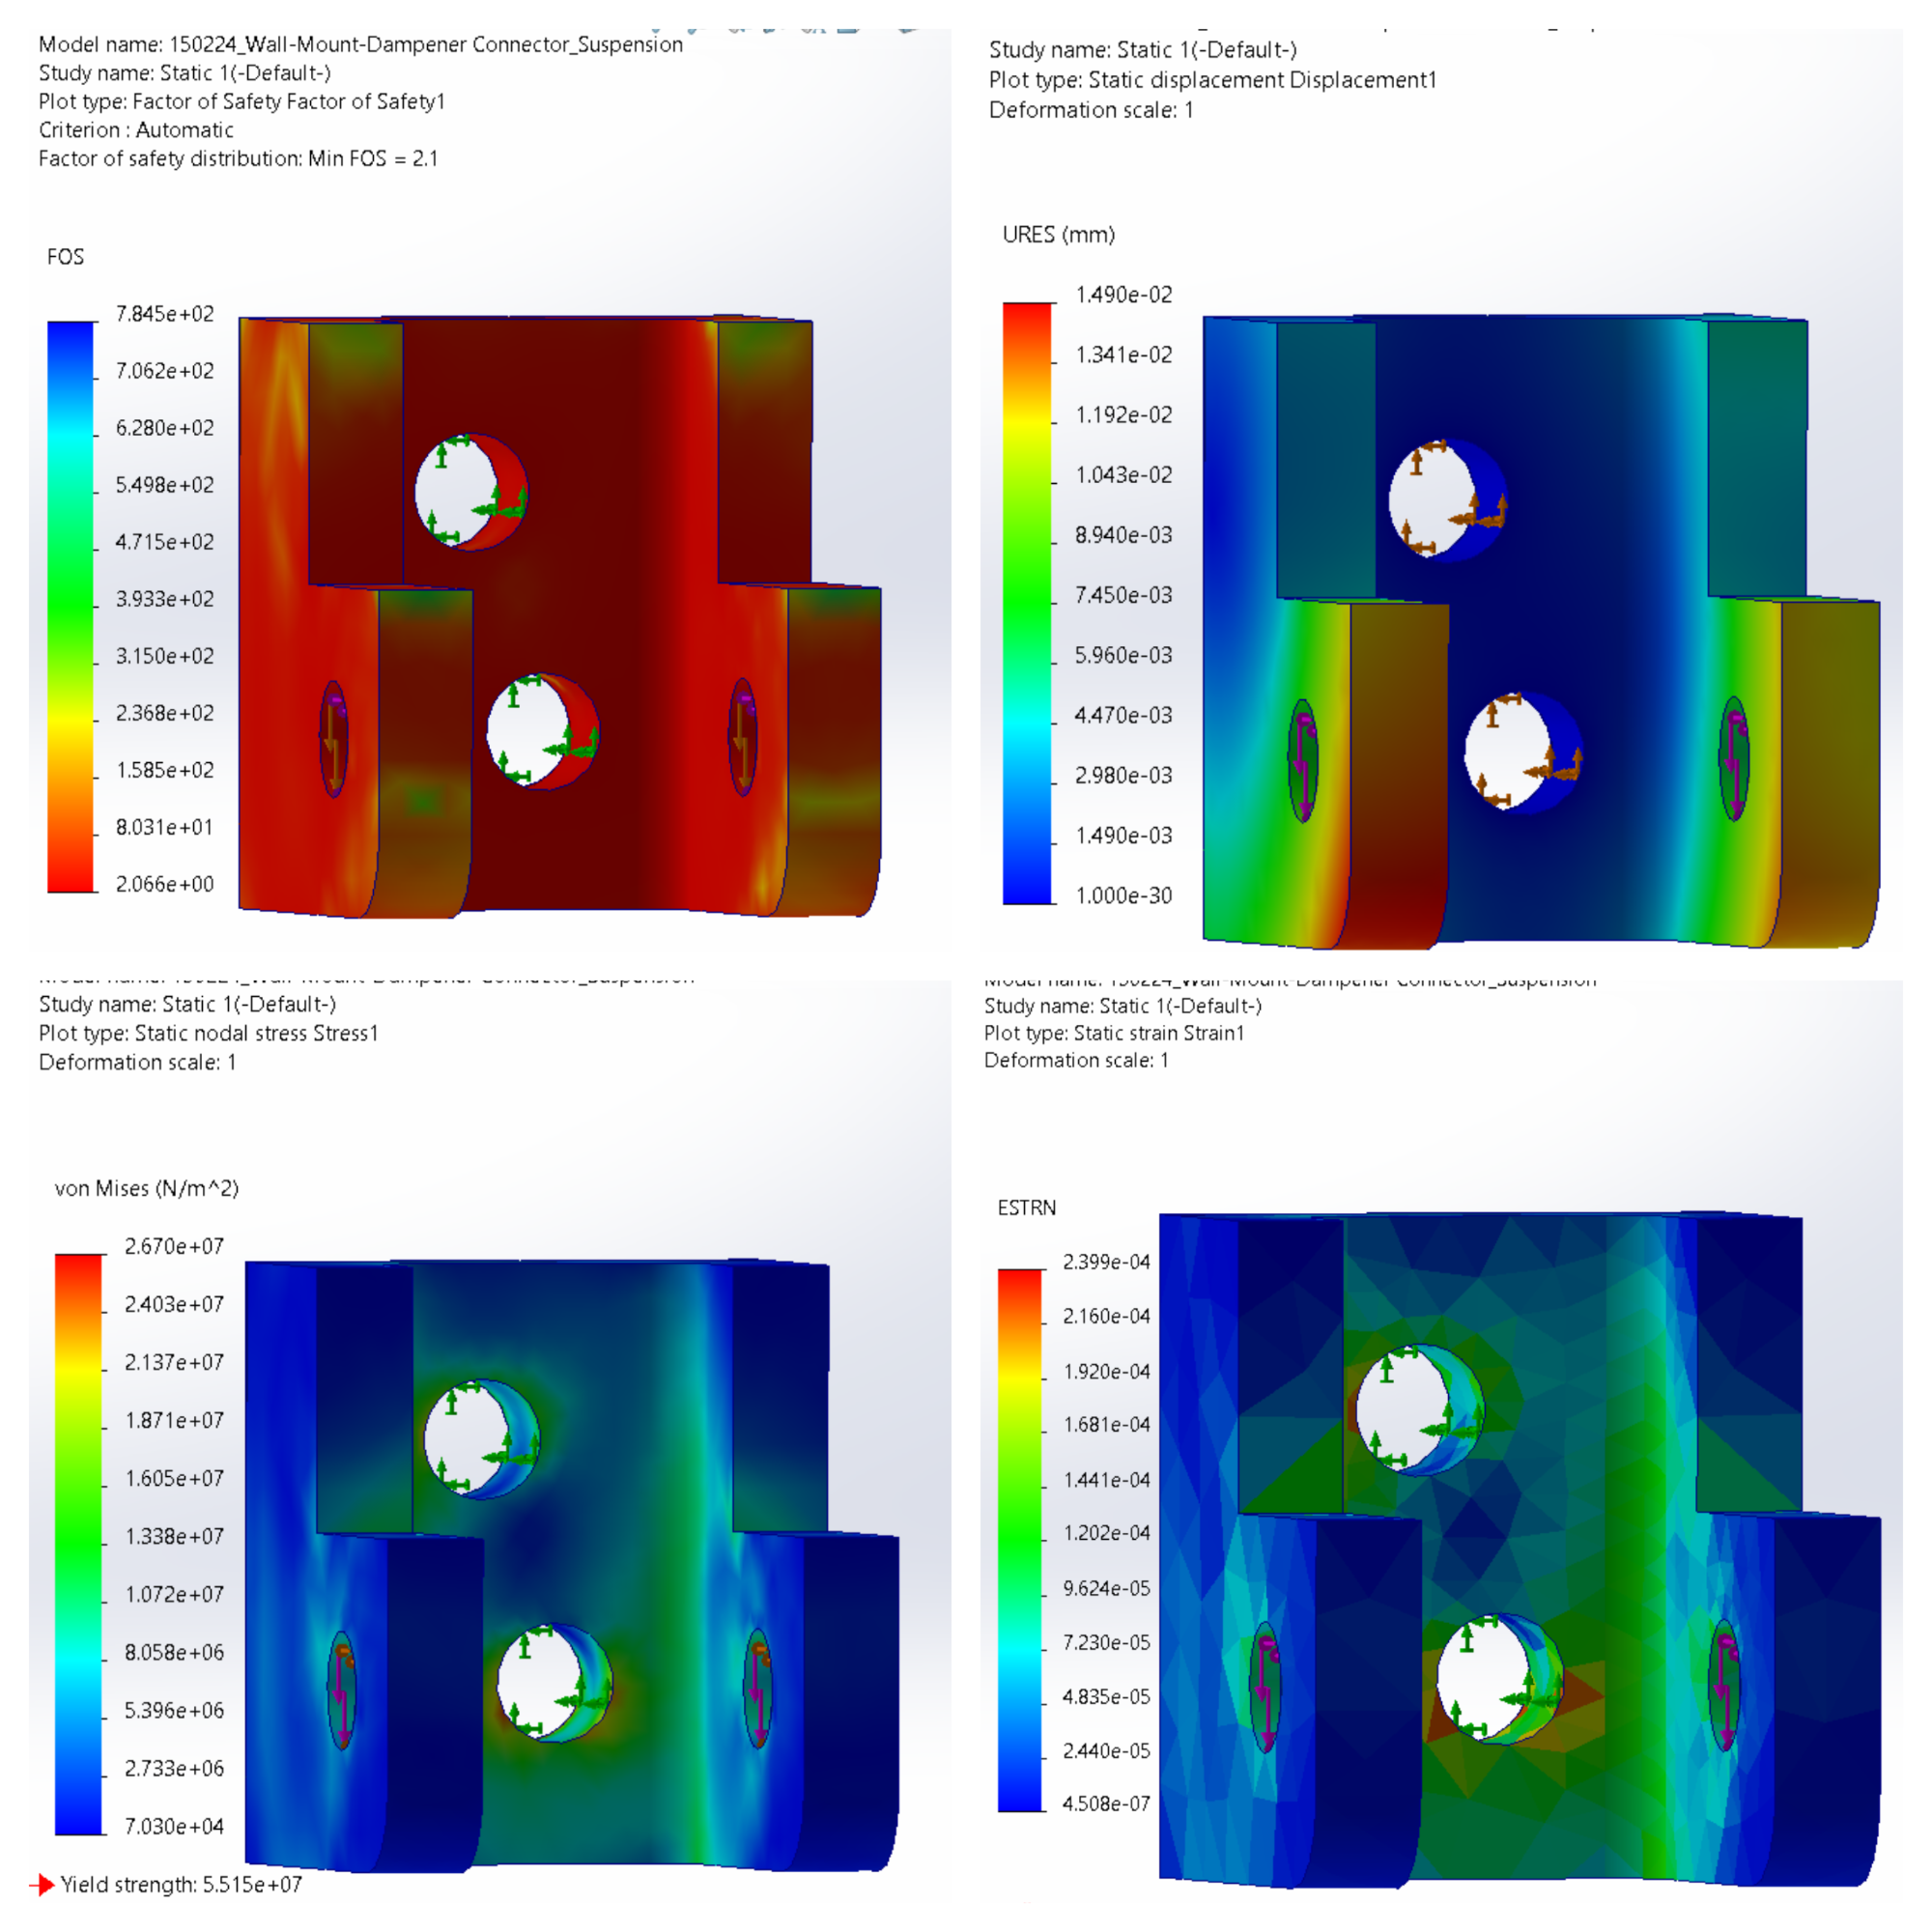
\includegraphics[width=\linewidth]{texfiles/mech/eimg/suspension/Mounting FEM results.png}
  \caption{Caption for the image.}
  \label{fig:image1}
\end{figure}


\begin{table}[H] % <-- Use [H] option to place the table exactly here
\centering
\caption{Mesh Information - Details}
\begin{tabular}{@{}ll@{}}
\toprule
\textbf{Parameter} & \textbf{Value} \\
\midrule
Total Nodes & 7097 \\
Total Elements & 4125 \\
Maximum Aspect Ratio & 6.3707 \\
\% of Elements with Aspect Ratio $<$ 3 & 99.2 \\
\bottomrule
\end{tabular}
\end{table}

This study presents a Finite Element Analysis (FEA) conducted to evaluate the structural integrity and performance of the shock absorber mounting configuration on the knuckle of a rear double wishbone suspension system. The primary objective was to assess the adequacy of the mounting design in withstanding applied forces and ensuring safety during operation. Initial simulations revealed areas of concern regarding the thickness of the mounting, prompting adjustments to the design parameters. Subsequent iterations were carried out to optimize the configuration, resulting in a revised model with enhanced strength characteristics. Through comprehensive analysis, a safety factor of 2 was achieved, indicating satisfactory resistance to anticipated loads. The findings of this study contribute to the understanding of structural behavior in automotive suspension systems and inform design improvements for enhanced performance and reliability (see Figure~\ref{fig:figure1}).




\newpage
\subsection{Manufacturing Process}
\subsubsection{Compilation of Parts List}
\begin{table}[H]
\centering
\caption{Component Specifications}
\begin{tabular}{|l|l|l|l|l|l|}
\hline
\textbf{Component} & \textbf{Number [-]} & \textbf{Mass [kg]} & \textbf{Size [mm x mm x mm]} & \textbf{Material} & \textbf{Manufacturing process} \\ \hline
Rear Wheels & x2 & - & $\phi$ 200 x 155 & Aluminum Alloy 6061 & In-house \\ \hline
Front Wheels & x2 & - & $\phi$ 200 x 50 & Galvanized Steel & Rollenplus.de (Outsourced) \\ \hline
Rear Knuckle & x2 & 1.473 & $\phi$ 145 x 52 & Aluminum Alloy 6061 & In-house \\ \hline
Cylindrical Roller Bearing Rear Knuckle & x4 & - & $\phi$ 85 x 18.6 & 100Cr6 & Outsourced \\ \hline
Retaining Ring DIN 472 & x4 & - & $\phi$ 85 & Spring Steel & Mädler (Outsourced) \\ \hline
Rear Upper Wishbone & x2 & 0.08896 & 119 x 102 x 6 & Aluminum Alloy 6061 & In-house \\ \hline
Rear Lower Wishbone & x2 & 0.1255 & 224 x 102 x 6 & Aluminum Alloy 6061 & In-house \\ \hline
Shock Absorber & x4 & - & $\phi$ 45 x 150 & - & XLC (Outsourced) \\ \hline
Wishbone Wall Mount & x16 & 0.02441 & 36 x 30 x 18 & Aluminum Alloy 6061 & In-house \\ \hline
Knuckle Wishbone Mount & x8 & 0.02055 & 37 x 25 x 18 & Aluminum Alloy 6061 & In-house \\ \hline
Rear Shock Absorber Mounts & x4 & 0.05583 & 40 x 40 x 35 & Aluminum Alloy 6061 & In-house \\ \hline
Linkage Mounts & x8 & 0.0135 & 31.75 x 22 x 18 & Aluminum Alloy 6061 & In-house \\ \hline
Female Rod End Bearing & x8 & - & 47 x 16 x 14 & Stainless Steel 1.4301 & Mädler (Outsourced) \\ \hline
Linkage Connecting Rod & x4 & 0.0032 & $\phi$ 7 x 43 & Aluminum Alloy 6061 & In-house \\ \hline
Uni Ball Bearings & x24 & - & $\phi$ 16 x 9 & 100Cr6 & Mädler (Outsourced) \\ \hline
Front Wheel Hub & x2 & 0.10959 & $\phi$ 40 x 115 & Aluminum Alloy 6061 & In-house \\ \hline
Front Wishbones & x2 & 0.09553 & 224 x 102 x 6 & Aluminum Alloy 6061 & In-house \\ \hline
Front Knuckle & x2 & 0.65721 & $\phi$ 160 x 15 & Aluminum Alloy 6061 & In-house \\ \hline
Front Shock Absorber Mounts & x4 & 0.01952 & 36 x 32 x 28 & Aluminum Alloy 6061 & In-house \\ \hline
Retaining Ring DIN 471 & x2 & - & $\phi$ 11 & Spring Steel & Mädler (Outsourced) \\ \hline
\end{tabular}
\end{table}

\subsubsection{Description of Efforts for Realistic Manufacturability}

Efforts for realistic manufacturability focus on optimizing production processes for critical suspension components, ensuring precision, reliability, and cost-effectiveness. This includes employing advanced manufacturing techniques and methodologies tailored to specific components, enhancing both efficiency and quality throughout the production process.

\subsubsection{Explanation of Manufacturing Techniques}


\textbf{Knuckle Manufacturing:} For the knuckle manufacturing process, a combination of water jet spray technology and CNC machining will be employed to ensure precise fabrication of critical features. The main hole for the shaft will be created using water jet spray technology, guaranteeing accuracy and efficiency in alignment and fitment. Additionally, advanced CNC machining will be utilized for creating internal grooves within the knuckle to accommodate the cylindrical roller bearings, ensuring precise dimensions and tolerances for proper seating and functionality of components.

\textbf{Wishbone Manufacturing:} Wishbones will be manufactured utilizing water jet spray technology, allowing for precise cutting of materials and efficient production. This ensures uniformity and consistency in the manufacturing process, resulting in high-quality wishbones that meet strict performance standards.

\textbf{Linkage Rod Manufacturing:} The linkage rod will undergo precision threading using a lathe machine, ensuring accurate fitment and functionality within the suspension system. This process guarantees precise dimensions and threading specifications, essential for seamless integration and optimal performance.

\textbf{Mountings:} Mountings on the knuckle assembly will be created using CNC machining, ensuring precise positioning and attachment of suspension components such as wishbones and shock absorbers. Additionally, the cylindrical roller bearings, facilitating specific movement within the knuckle, will be press-fitted to ensure secure placement and alignment. This method ensures stability and longevity within the suspension system.

\subsection{Integration Process}
\subsubsection{Explanation of Integration with Other Subsystems}
\textbf{Integration with Other Subsystems:} Integration with other subsystems is essential for ensuring the seamless operation and optimal performance of the suspension system within the overall vehicle architecture. In our case, integration with the propulsion system has been a key focus, particularly due to the presence of a shaft in the suspension design. This integration involves several considerations, including the offset positioning of the shock absorber to accommodate the shaft.

\textbf{Shaft Integration:} The presence of a shaft within the suspension system necessitates careful consideration to ensure compatibility with other vehicle subsystems, particularly the propulsion system. The shaft may be part of the drivetrain, connecting the engine or motor to the wheels for propulsion. Integration with the suspension requires accommodating the shaft's presence without compromising the functionality or performance of either system.

\textbf{Offset Shock Absorber Positioning:} To accommodate the shaft within the suspension assembly, the positioning of the shock absorber may need to be offset from its conventional location. This offset positioning ensures clearance between the shock absorber and the shaft, preventing interference and maintaining the integrity of both systems. By strategically adjusting the shock absorber position, we ensure optimal functionality of the suspension while accommodating the requirements of the propulsion system.

\textbf{Integration with Braking System:} In addition to integration with the propulsion system, seamless integration with the braking system is vital for overall vehicle performance and safety. Specifically, considerations have been made to ensure that the braking pads remain 7mm below the track surface for effective braking. This requirement has been addressed by utilizing an adjustable shock absorber design. By adjusting the shock absorber, we can precisely control the ride height of the vehicle, thereby maintaining the desired clearance for the braking system. This integration ensures that braking performance is not compromised and contributes to the overall safety and functionality of the vehicle.

By integrating the suspension system with the propulsion and braking systems, we achieve synergies that enhance overall vehicle performance, handling, and ride comfort. This integration optimizes the utilization of space within the vehicle, maximizes efficiency, and ensures compatibility between critical subsystems. Additionally, it reflects our commitment to engineering solutions that prioritize functionality, reliability, and seamless operation across all vehicle systems.



\section{Braking}
The brake system in a vehicle is undeniably one of its most critical components, serving the vital function of controlling its speed and ensuring safe stops when necessary.


\subsection{Overview}
With various types of braking systems available:

\begin{itemize}
    \item Mechanical Brake System
    \item Hydraulic Brake System
    \item Pneumatic Brake System
    \item Electromagnetic Brake System
    \item Electrical Brake System
    
\end{itemize}

Among these options, we have opted to implement the pneumatic braking system due to its simplicity in construction and its ability to provide a fail-safe mechanism through selection types. Pneumatic brakes offer reliable performance and can be well-suited for various vehicle applications, particularly those requiring robust and efficient braking capabilities.
\subsubsection{Requirements and Constraints}
In designing and implementing a vehicle's braking system or pod, careful attention is put on specific requirements and considerations. The complex design for the braking system of a pod depends largely on the maximum speed that can be achieved by the vehicle. Faster speeds call for finer brake parts to allow for proper and safe deceleration hence putting more emphasis on exactness in the system design. On top of this, knowing how much energy that is stored in it is vital to ensure safe braking operations. It is therefore important to discharge this energy properly during braking so as to avoid overheating, mechanical failure, and to preserve the reliability of this system.\\


Moreover, there are certain restrictions to be followed in order for the braking process to be effective. These also include handling efficiently static weight of the pod plus any additional loads experienced during operation. Also, it should be designed with respect to high vehicle speed when considering stopping power within a reasonable range for safety purposes of passengers. Knowledge about distance required stopping is very significant here; such that brakes are made so as they can safely cause deceleration within that distance hence preventing accidents from happening.By adhering meticulously to these requirements and constraints, a braking system can be designed and implemented effectively, ensuring the safety and optimal performance of the pod.

\subsubsection{Concept}
Our major objective is simple: to develop a brake system that can never fail, guaranteeing the highest level of dependability and safety. Important components of the system include actuators, springs, and a pneumatic system. The pre-compressed springs provide the majority of the braking force, while the pneumatic system and actuators help in controlling and holding them in position.
Because a pneumatic system reacts rapidly, which is essential for effective braking, we decided to retract the spring using it. Although we might think about utilizing electrical actuators, their cost is prohibitive and would necessitate a large budget adjustment for the entire pod. For the purposes of our project, the pneumatic technique makes the most sense.





\section{Size, Components, and Appearance}

\begin{table}[htbp]
\centering
\begin{adjustbox}{width=\textwidth} % Adjust table width to fit textwidth
\begin{tabular}{|c|c|c|c|c|c|}
\hline
\textbf{Component} & \textbf{Number} & \textbf{Mass [g]} & \textbf{Size [mm]} & \textbf{Material} & \textbf{In-house/Outsourced} \\
\hline
\textbf{Main Spring} & $\times$16 & 3163.2 & - & - & - \\
\textbf{Brake Pad} &$\times$16 & 406.4 & - & - & - \\
\textbf{Pad Mounting Bracket} & $\times$4 & 2296.6 & - & - & - \\
\textbf{Big Actuator} & $\times$4 & 8868 & - & - & - \\
\textbf{Small Actuator} &$\times$8 & 2432 & - & - & - \\
\textbf{Tube 8mm} & $\times$5 & - & - & - & - \\
\textbf{Tube 6mm} &  $\times$1.5 & - & - & - & - \\
\textbf{Tube 4mm} &  $\times$1.5 & - & - & - & - \\
\textbf{Tube adapter 4-8} &$\times$6 & - & - & - & - \\
\textbf{Tube adapter 6-8} & $\times$4 & - & - & - & - \\
\textbf{X-connector 8mm} &$\times$2 & - & - & - & - \\
\textbf{T-connector 8mm} & $\times$10 & - & - & - & - \\
\textbf{Pressure regulator} &$\times$2 & - & - & - & - \\
\textbf{Pressure tank} &$\times$2 & - & - & - & - \\
\textbf{Pressure sensor} & $\times$8 & - & - & - & - \\
\textbf{Main valve} &$\times$2 & - & - & - & - \\
\textbf{Venting valve} &$\times$2 & - & - & - & - \\
\textbf{Manometer} & $\times$2 & - & - & - & - \\
\textbf{One way valve (adjustable)} &$\times$2 & - & - & - & - \\
\textbf{Proximity sensor} & $\times$4 & - & - & - & - \\
\textbf{Sensor adapter cable} &$\times$8 & - & - & - & - \\
\textbf{Light barrier} & $\times$2 & - & - & - & - \\
\textbf{Distance sensor} & $\times$2 & - & - & - & - \\
\textbf{Tank and PR adapter} & $\times$8 & - & - & - & - \\
\textbf{Main actuator adapter} & $\times$2 & - & - & - & - \\
\textbf{Side actuator adapter} &$\times$4 & - & - & - & - \\
\textbf{Manometer adapter} & $\times$4 & - & - & - & - \\
\textbf{Pressure sensor bracket} & $\times$8 & - & - & - & - \\
\textbf{One way valve bracket} & $\times$2 & - & - & - & - \\
\textbf{IO-Link® master USB} &$\times$1 & - & - & - & - \\
\textbf{IO-Link® master USB cable} & $\times$1 & - & - & - & - \\
\textbf{Blanking plug 8mm} & $\times$2 & - & - & - & - \\
\textbf{Muffler 8mm} & $\times$4 & - & - & - & - \\
\textbf{Multiple hose clamping bar} & $\times$2 & - & - & - & - \\
\textbf{Thread sealing tape} & $\times$1 & - & - & - & - \\
\textbf{Cable binders} & $\times$10 & - & - & - & - \\
\textbf{Brake Mounting} & $\times$2 & - & - & - & - \\
\hline % Add horizontal line here for first three columns
\multicolumn{2}{|c|}{\hspace{3cm}\large\textbf{Total Weight}} & \\
\cline{1-3} % Only for the first three columns
\end{tabular}
\end{adjustbox}
\caption{Components and Manufacturing Details}
\label{table:components}
\end{table}








\newpage
\subsection{Theoretical concepts}
\label{subsec:theoretical-concept}
The sequence of events is triggered when you apply the brakes in the pneumatic brake system.The compressed springs are already in place and ready to go when the system is first supplied with compressed air.\\

The actuator piston is forced forward when you apply the brakes because the brakes send out a signal to release compressed air.Converting the compressed air's energy into mechanical energy to powers this movement.\\

In tandem, the pre-compressed spring expands and pushes the actuator piston further as the air pressure decreases.
In order to create the necessary friction to slow down the vehicle, the expanding spring and the moving piston work together to bring the brake pad into contact with the braking surface.
\subsection{Design Process and Appearance}
Taking into account variables like weight, speed, and stopping distance is the first step in the system design process. According to the given parameters, the pod's target weight is 250 kg, and its top speed is 60 km/h. The pod must be able to be stopped with sufficient force by the braking mechanism. Currently, our solution satisfies this criteria by guaranteeing that the pod may stop fully within a 20.5 m.



\subsubsection{CAD Models and Technical }
\begin{figure}[!ht]
  \centering
  \begin{minipage}[b]{0.45\linewidth}
    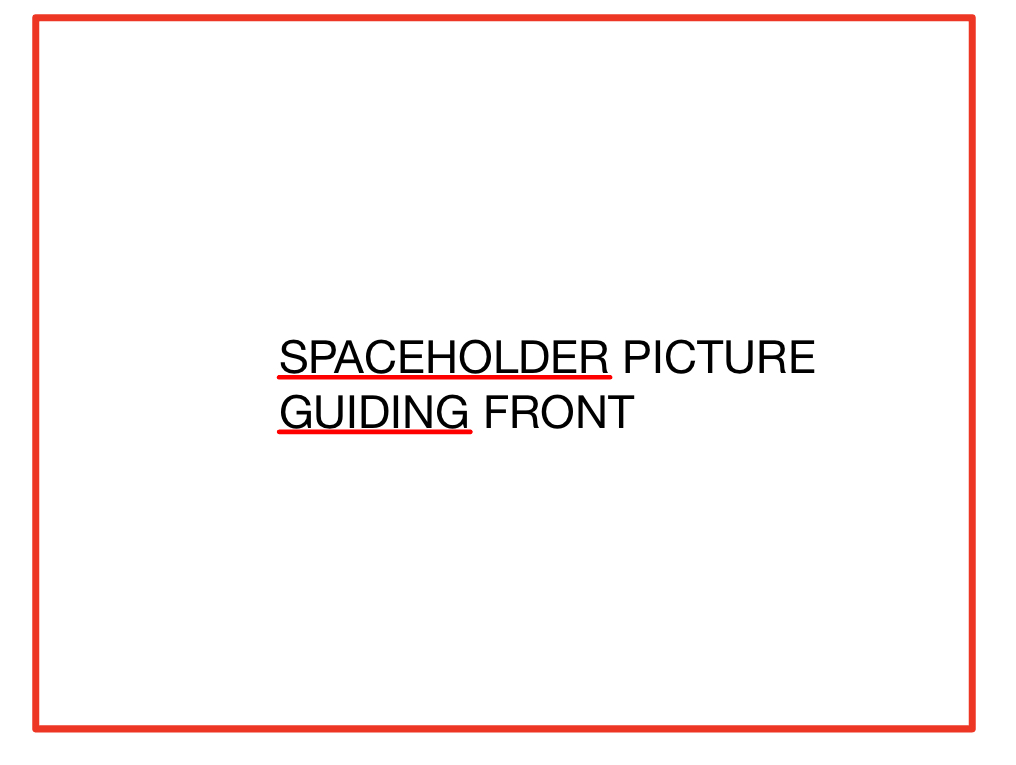
\includegraphics[width=\linewidth]{texfiles/mech/eimg/braking/guiding_front_1.jpg}
    \caption{CAD Guiding Front}
    \label{fig:guiding_front}
  \end{minipage}
  \hspace{0.5cm}
  \begin{minipage}[b]{0.45\linewidth}
    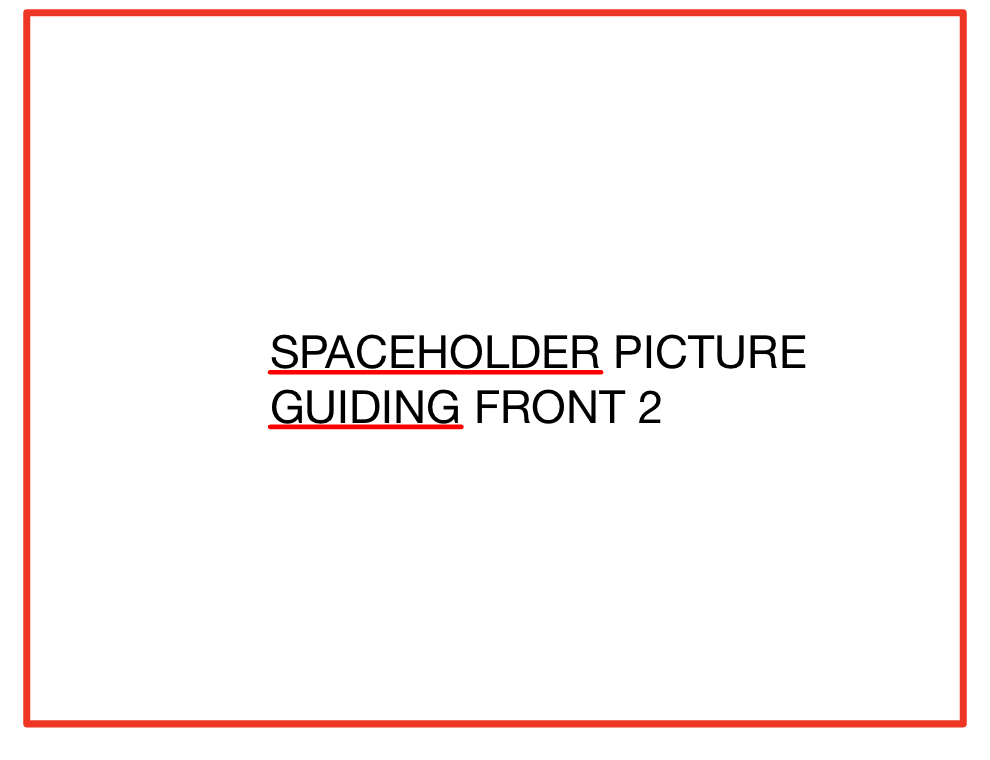
\includegraphics[width=\linewidth]{texfiles/mech/eimg/braking/guiding_front_2.jpg}
    \caption{CAD Guiding Rear}
    \label{fig:guiding_rear}
  \end{minipage}
\end{figure}

\begin{figure}[!ht]
  \centering
  \begin{minipage}[b]{0.45\linewidth}
    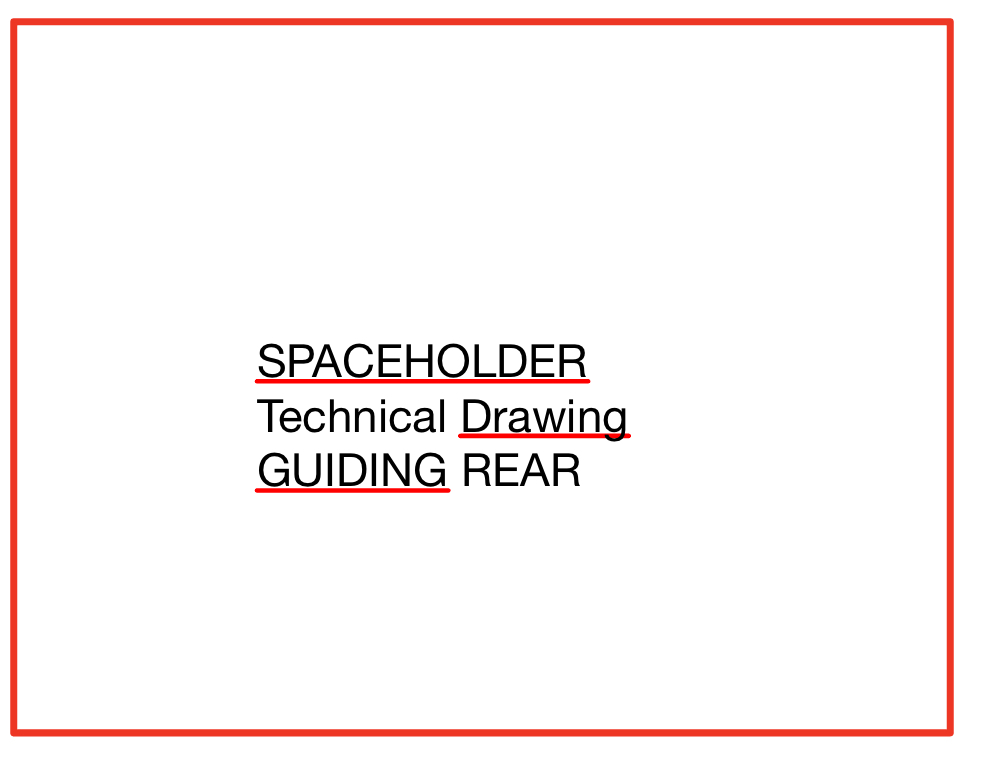
\includegraphics[width=\linewidth]{texfiles/mech/eimg/braking/guiding_tech_rear.jpg}
    \caption{CAD Guiding Front \#2}
    \label{fig:guiding_front_2}
  \end{minipage}
  \hspace{0.5cm}
  \begin{minipage}[b]{0.45\linewidth}
    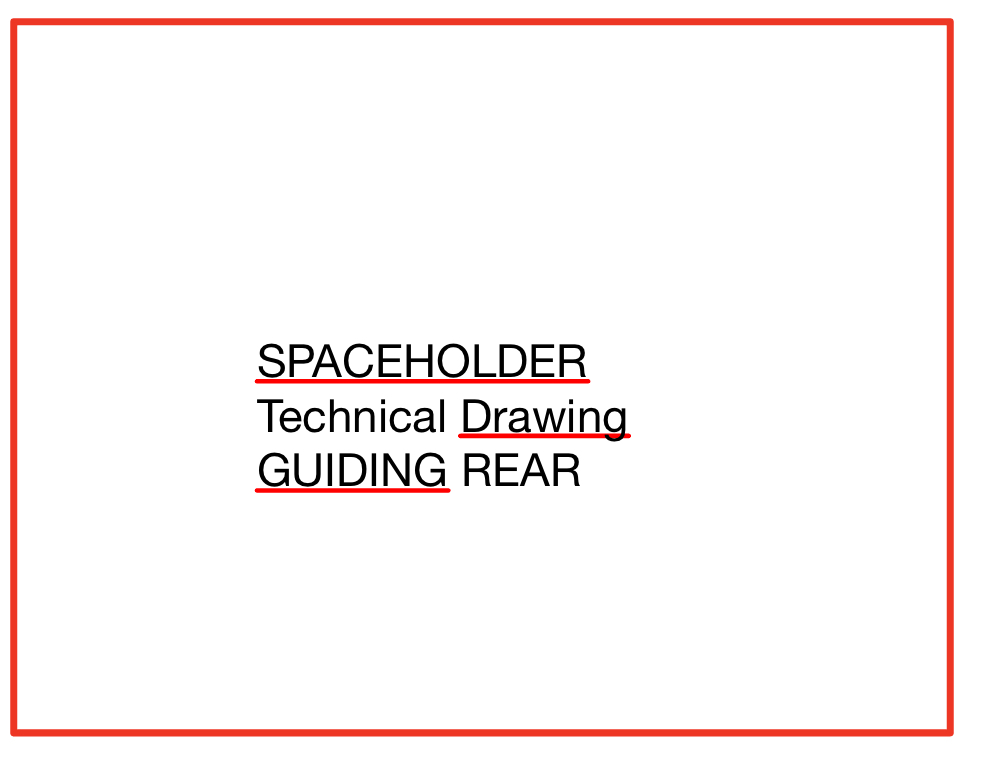
\includegraphics[width=\linewidth]{texfiles/mech/eimg/braking/guiding_tech_rear.jpg}
    \caption{CAD Guiding Rear 2}
    \label{fig:guiding_rear_2}
  \end{minipage}
\end{figure}

\begin{figure}[!ht]
  \centering
  \begin{minipage}[b]{0.45\linewidth}
    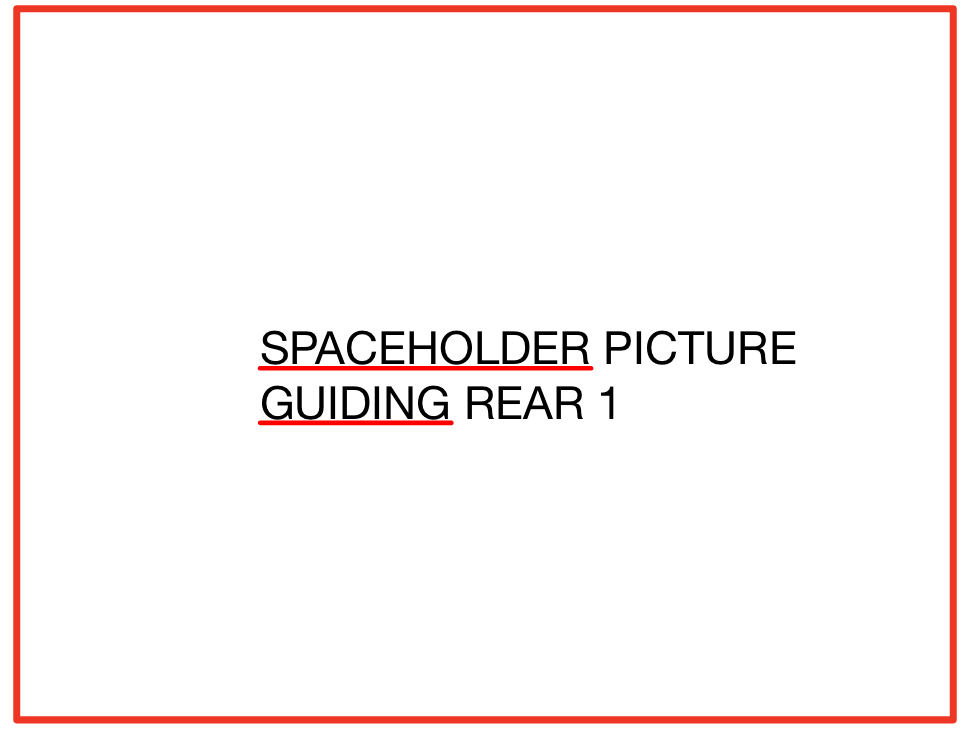
\includegraphics[width=\linewidth]{texfiles/mech/eimg/braking/guiding_rear_1.jpg}
    \caption{Technical Drawing Guiding Front }
    \label{fig:guiding_front_2}
  \end{minipage}
  \hspace{0.5cm}
  \begin{minipage}[b]{0.45\linewidth}
    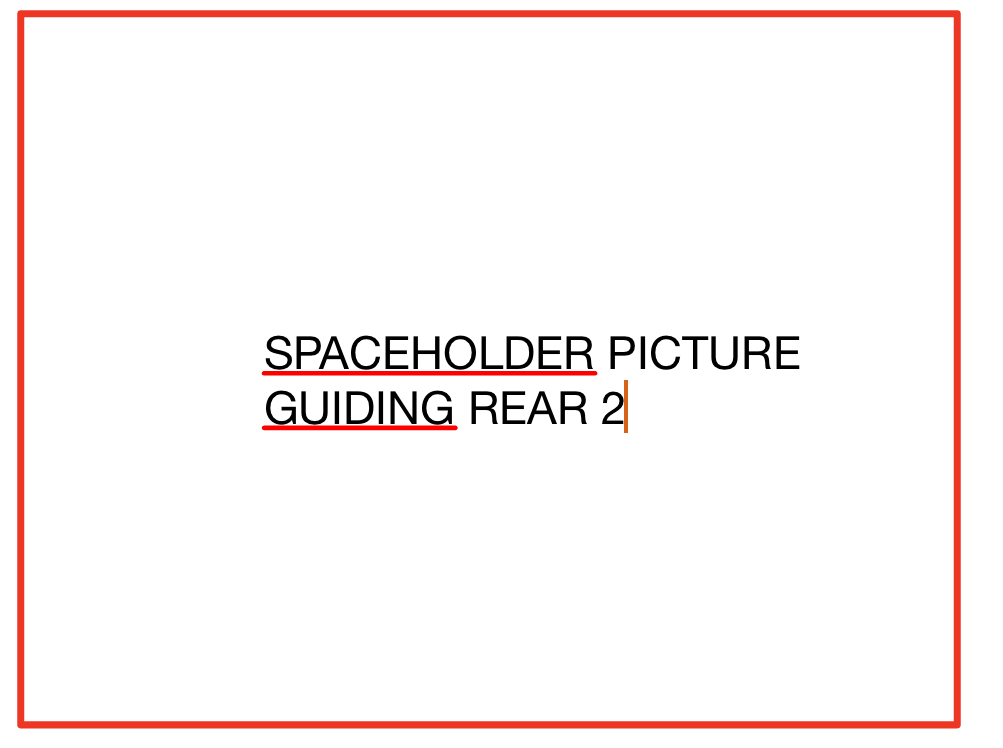
\includegraphics[width=\linewidth]{texfiles/mech/eimg/braking/guiding_rear_2.jpg}
    \caption{Technical Drawing  Guiding Rear}
    \label{fig:guiding_rear_2}
  \end{minipage}
\end{figure}

\newpage
\subsubsection{Materials}
To ensure maximum performance and longevity, the materials used for the subsystem components specifically, the small actuator mounting and the large brake mounting have been carefully chosen.  The choice of plain carbon steel can be attributed to its superior mechanical properties, affordability, and suitability for its intended application. It's also simple to work with and shape during production, which lowers costs and promotes efficient production.


Because plain carbon steel is durable and resistant to corrosion, it can withstand extreme conditions and last for a very long time. It is very easy to weld, which makes assembly simpler.

Finding the ideal mix between strength, the lifespan, ease of manufacture, and cost-effectiveness was the main consideration in the selection of plain carbon steel for these components.

\subsubsection{Design Rationale}
The main goal of the braking system design is to use advanced design ideas and make sure the pod can stop completely within predetermined parameters.

The design's fundamental idea is to use springs to provide a fail-safe mechanism. Our goal in using springs is to create a braking mechanism that can operate even in the case of a leak or system failure. The unique part is how the actuators are used to keep the springs compressed by operating in reverse. This design element strengthens the system's fail-safe capability by guaranteeing that the pod can activate braking even in the event of a malfunction or physical damage.
In conclusion, the braking system's creative use of actuators that operate in reverse and relying on springs are designed to promote safety and dependability. This method guarantees that even in difficult situations, the pod can brake within predefined limits. 
\subsubsection{FEM Results}
.  Present FEM results for worst-case scenarios, including images and values.
\paragraph{\Large{Calculations:}}






\begin{itemize}[leftmargin=*]
    \item[$\bullet$] \textbf{Kinetic Energy}
\end{itemize}

\noindent
For a pod with mass \(m=260\ \text{kg}\) and speed \(v=70\ \text{km/h}\), \textbf{kinetic energy} is defined as
\begin{align*}
    E_k &= \frac{1}{2} mv^2
\end{align*}
Substituting the given values:
\begin{align}
    E_k &= \mathbf{49151} \, \textbf{J}
\end{align}













\begin{itemize}[leftmargin=*]
  \item[\hspace{-1cm}$\bullet$] \textbf{Braking Force}
\end{itemize}
\noindent
To stop the pod within a certain distance, we must account for the work done to compensate for its kinetic energy. According to the principle of work, when an object moves against a force exerted on it, work is done. Specifically, if the object moves through a displacement $d$ while experiencing a constant force $F$, the force performs an amount of work given by




\[
W = F \cdot d
\]

To find the force \( F \) exerted on the pod, given that the work done is \( W = 49151~\text{J} \) and the stopping distance is \( d = 20~\text{m} \), we rearrange the formula:

\begin{align}
F &= \frac{W}{d} \notag \\
\textbf{Braking force } F &= \mathbf{2457.6}\, \textbf{N} 
\end{align}







\begin{itemize}[leftmargin=*]
    \item[$\bullet$] \textbf{Normal Force}
\end{itemize}
\noindent
To determine the required normal force exerted on the brake pads in order to achieve the necessary brake force, consideration must be given to the coefficient of friction ($\mu = 0.36$) between the brake pads and the track surface.






The required normal force (\( N \)) exerted on the brake pads can be calculated using the formula:

\begin{align}
    N &= \frac{F}{\mu} \notag \\     
  \textbf N  &= \mathbf{6826.66} \, \textbf{N}
\end{align}

where \( F = 2457.6 \) and \( \mu = 0.36 \).\\

The normal force per assembly, with consideration for two distinct assemblies, refers to the resultant force exerted perpendicular to the contact surfaces of each respective assembly.\\

\begin{equation}
\textbf{Normal force per assembly} = \mathbf{3413.28 \,N}
\end{equation}

\newpage
\begin{itemize}[leftmargin=*]
    \item[$\bullet$] \textbf{Spring Calculation}
\end{itemize}
\noindent
Given the parameters provided:

\begin{align*}
    \text{Resting length of the spring} (L_0) &= 187 \, \text{mm} \\
    \text{Spring constant} (k) &= 5.97 \, \text{N/mm} \\
    \text{Compressed length of the spring} (L_1) &= 94 \, \text{mm} \\
    \text{Actuator length} (L_{\text{actuator}}) &= 92 \, \text{mm} \\
    \text{Spring used in mounting} (L_{\text{mounting}}) &= 2 \, \text{mm}
\end{align*}
\noindent
When the spring is compressed from its resting length to the compressed length:

\begin{align*}
    \text{Initial Force} (F_{\text{initial}}) &= k \times (L_0 - L_1) \\
    &= 5.97 \times (187 - 94) \, \text{N} \\
    &= 555.21 \, \text{N}
\end{align*}
\noindent
Upon expansion of the spring to accommodate braking, extending to a length of 114 mm:

\begin{align*}
    \text{Force Required} (F_{\text{expansion}}) &= k \times (L_0 - L_{\text{braking}}) \\
    &= 5.97 \times (187 - 114) \, \text{N} \\
    &= 435.81 \, \text{N}
\end{align*}
\noindent
Since each assembly utilizes 8 springs, the total force required for both assemblies is:

\begin{equation}
\begin{aligned}
    \text{Total Force} (F_{\text{total}}) &= \text{Number of springs} \times F_{\text{expansion}}\notag \\
     \end{aligned}
\end{equation}
\begin{equation}
   \mathbf{Total\ Force} = \mathbf{6972.96 \, N}
\end{equation}



Considering the total normal force of 6826.66 N, it appears that the calculated force from the springs exceeds the total normal force, indicating that the system can function properly under these conditions.



\begin{itemize}[leftmargin=*]
    \item[$\bullet$] \textbf{Actuator Force}
\end{itemize}

\noindent
To determine if the chosen actuators can effectively compress and hold the springs to meet the normal force requirement, we need to calculate the total force capacity provided by all actuators. Given that we have 2 big actuators and 4 small actuators, each with a capacity of 686 N (at 6 bar pressure), we can calculate the total force capacity for each assembly:

\[
\textbf{Total force capacity} = \mathbf{4116} \, \textbf{N}
\]

Comparing this with the required normal force of 3413.28 N, we can see that the total force capacity provided by the actuators exceeds the requirement. Therefore, the chosen actuators are sufficient to compress and hold the springs to achieve the desired normal force on the track surface.

\newpage
\begin{itemize}[leftmargin=*]
    \item[$\bullet$] \textbf{Actuator Pressure}
\end{itemize}
\noindent
Given that the system can handle pressures between $6$ to $10$ bar, with $P_1 = 6$ bar and $F_1 = 686$ N (as per the catalogue) where the actuator can exert a force of $686$ N at $6$ bar.\\

With $8$ springs per assembly and a previously calculated compressed spring force of $555.21$ N, the total compressed spring force per assembly is $8 \times 555.21 = 4441.68$ N.\\
\noindent
Utilizing $6$ actuators per assembly, the required force from each actuator is 
\[
F_2 = 740.28 \, \text{N}.
\]

Now, let's calculate the pressure required for the actuators to handle this force: \\
 
- Using the formula $F = P \times A$, where $F_1 = P_1 \times A$ and $F_2 = P_2 \times A$.\\  
\[
P_2 = \frac{P_1 \times F_2}{F_1}.
\]  

- Substituting the given values, 
\begin{equation}
\mathbf{P_2} = \mathbf{6.47} \, \textbf{bar}.
\end{equation}

Hence, the pressure required for the actuators to handle this condition is approximately $6.5$ bar.
\subsubsection{Mesh and Boundary Conditions}
.  Provide details on the type of mesh, boundary conditions, and Free Body Diagrams.


\subsection{Manufacturing Process}
Kindly consult \textbf{Table \ref{table:components}} for reference.\\

\noindent
We've taken steps to ensure that our braking system is more than just a concept and can be manufactured realistically.\\

\noindent
\textbf{Selecting Materials Which Are Easy to Use}: The materials utilized for each component were selected based on their availability and convenience of production for the intended use. for instance, Carbon steel and other common metals, are chosen due to their easy production and wide availability.\\

\noindent
\textbf{Using Standard Parts}: We made an effort to use components that are widely available and simple to assemble, such as tubes, connectors, and adapters. As a result, producers can assemble everything more easily and without the need for specialized tools.\\ 

\noindent
\textbf{Assembly Ease}: The complete brake system's assembly has been taken into consideration. Parts are made to fit together easily, and assembly workers are assisted by clear labelling and instructions when needed.



\subsection{Integration process}
\subsubsection{Assembling}
Bolts will be used to firmly secure the main brake system to the chassis. Then, using specific mounts, small actuators will be fastened to the brake assembly.

Bolts will then be used to secure the aluminium brackets to the actuators. Before pressurizing the system, springs will be positioned between the metal brackets.




\subsubsection{Assembly interaction}
The longitudinal and lateral planes of the chassis must be securely fastened to the main mounting bracket. In in addition to providing structural support to the central section of the chassis, that connection will transmit forces to the chassis, resulting in the creation of a complete system.



\subsection{Safety Considerations}
\subsubsection{Safety Factor}
\textbf{Selecting Strong Materials:} Parts that make up pneumatic brakes, such as brake housings and valves, are made of hard materials such as steel and reinforced rubber These materials can withstand during braking.\\

\noindent
\textbf{To handle pressure safely:} Air brake systems operate under high pressure, so the parts are designed to handle much higher pressures than they will actually experience during normal use This additional capability this ensures that the system remains safe even if pressure fluctuations or screws occur.\\

\noindent
\textbf{Passing safety tests:} All parts in an air brake system go through rigorous tests to ensure they meet safety standards. These tests test things like how well the parts hold up under stress and whether they perform well under different conditions.\\

\noindent
\textbf{Backup system:} Many brake systems have a built-in backup system. For example, if one part fails, there is usually another part that can take over, ensuring that the brakes remain functional in an emergency. In our case, springs are used to create a brake mechanism that can operate even in the event of a leak or system failure. 
\subsubsection{Worst-Case Scenarios}

It can be dangerous to rely solely on air pressure in a standard pneumatic braking system without a fail-safe feature if the pressure drops unexpectedly or if there is a malfunction with the system.  \\

 \noindent
\textbf{Worst case scenario without Fail safe mechanism:}
This system only relies on air pressure. Leak of air or mechanical problem cause the air suddenly disappears, the brake might fail when needed. This makes accidents more likely.\\

\noindent
\textbf{Adding a Fail safe mechanism:}
if there is a problem with air pressure or  in case might be drop, this fail safe feature turns on by itself. it makes sure the brakes keep working even if pressure drop.

\subsection{FMEA Results Discussion}
\subsubsection{Risk Assessment}
.  Preliminary risk assessment for demonstration, transport, and lifting.
\subsubsection{FMEA and Risk Mitigation}
.  Detail FMEA and describe risk mitigation measures.
\subsubsection{Simulation Evidence}
.  Provide evidence of simulations validating theoretical assumptions.


\subsection{Testing}
\subsubsection{Safety Procedures Documentation}
Testing Procedures for Pneumatic Brake System\\

\noindent
\textbf{Pre-Test Inspection:}
Ensuring Braking component are properly attached and free from leaks.\\
Check that the compressed springs are at right place and working properly.\\

\noindent
\textbf{Pressure Check:} With use of pressure gauge to measure the air pressure in the system.\\
Continue increase the pressure to the recommended operating level and check for any pressure drops before operating system.\\

\noindent
\textbf{Monitor the expansion of the spring:}
Verify the expansion of spring as the air pressure decreases.Check that the spring works in Simultaneously with the actuator piston to maintain proper braking force.
Finally, Conduct a final inspection of all components of the system to ensure they remain in good condition.\\

\noindent
\textbf{Activate the Braking system by giving signal:}Check how actuator piston react and check that it moves forward correctly.
verify that the brake pad makes proper contact with the braking surface to create the friction that can enough to slow down the pod.\\

\noindent
\textbf{By applying emergency Brake Test:}
If we have to stop the vehicle in emergency situation,by conducting an emergency brake to check that it can able to quickly stop the pod. 

\subsubsection{Preliminary testing plan}
As we discussed above preliminary testing plan for the pneumatic braking system involves several key tests to validate its functionality and performance.\\
The expected results include regularly pressure build-up, smoother movement of piston, spring expansion and enough friction of brake pad to slow down the vehicle and  Safety precautions will be implemented throughout the testing process to ensure a safe environment and prevent any potential risk.

\subsection{Additional considerations}
\noindent
\subsubsection{Pneumatic Braking System:}
\paragraph{Possible Failures:} Brake systems can malfunction in a number of ways. it include malfunctioning , worn brake pads, pneumatic system failures, air leaks, worn brake pads or discs, electrical issues,  mechanical damage and weather conditions. Regular inspection and maintenance are essential to ensure the system's reliability and safety.
\paragraph{Pressure Requirement:}We are filling the pneumatic system with a pressure of 6.5 bar, well within the system's handling capacity, which ranges between 6 to 10 bar. To ensure that the pressure remains within safe limits, we are using a filling tank and pressure regulator. These components prevent the pressure from exceeding the specified limits and ensure the pneumatic system operates safely and effectively.\\
  
	
\subsection{References}
%Picture of Pneumatic Circuit


\section{Eddy Current Braking}
\subsection{Introduction}
\subsubsection{FDD.9 Budget, Funding, and Manufacturing Methods}
 
\subsection{Technical Description and Constraints}
\subsubsection{FDD.11 Technical Specifications}
 
\subsubsection{FDD.17 Design Constraints}
 
\subsubsection{FDD.18 Performance Requirements}
 
\subsubsection{FDD.19 Integration with Other Systems}
 
\subsection{Objectives and Design Approach}
\subsubsection{FDD.12 Design Objectives}
 
\subsubsection{FDD.15 Innovative Aspects}
 
\subsubsection{FDD.16 Design Approach}
 
\subsection{Safety}
\subsubsection{FDD.13 Safety Considerations}
 
\subsubsection{FDD.14 Safety Testing and Compliance}
 
\subsection{Parts List (FDD.21)}
% Comprehensive list of all parts used in the braking system, including specifications and suppliers.

\newpage

\section{Aerodynamics}


\subsection{Overview}
The design of the Hyperloop pod aeroshell is meticulously crafted to optimize aerodynamic performance and ensure stability during high-speed travel. This section explores the key design considerations and features of the aeroshell subsystem, highlighting its role in reducing air resistance and enhancing the overall efficiency of the Hyperloop transportation system.

\subsubsection{Requirements and Constraints}
The Hyperloop pod aeroshell is required to fulfill several critical functions to ensure optimal performance of the transportation system. Firstly, it must minimize air resistance to facilitate smooth movement through the Hyperloop tube, thereby reducing energy consumption and increasing overall speed. Additionally, the aeroshell should enhance stability and control during acceleration, deceleration, and maneuvers, contributing to passenger comfort and safety. Furthermore, the design should incorporate features to manage airflow efficiently, preventing turbulence and ensuring a streamlined flow around the pod. Compliance with safety regulations and structural integrity are also paramount, ensuring the aeroshell can withstand operational stresses and environmental conditions encountered during Hyperloop travel.

\subsubsection{Concept}
The concept of the aeroshell subsystem revolves around maximizing aerodynamic efficiency while ensuring structural integrity and safety compliance. Inspired by proven aerodynamic principles, the aeroshell design prioritizes minimizing air resistance, enhancing stability, and facilitating controlled airflow. By incorporating features such as a streamlined front and rear configurations, the aeroshell optimizes performance while maintaining adherence to safety standards and regulatory requirements outlined in the Functional Design Description (FDD) for the Hyperloop competition.
\subsubsection{Size, Components, and Appearance}
.  Include a table of materials, mass, dimensions, and other relevant factors.
\begin{table}[ht]
\centering

\label{table:components}
\begin{adjustbox}{width=\textwidth,center}
\begin{tabular}{|>{\bfseries}m{2.5cm}|m{1.4cm}|m{1.7cm}|m{2.1cm}|m{2.2cm}|m{2.6cm}|m{2.2cm}|}
\hline
Component & Number & Mass [kg] & Size [mm] & Material & Manufacturing process & In-house/ outsourced \\
\hline
Wheels & x8 & 1 & 100 x 50 & Polyurethane & Injection molding & Outsourced \\
Axles & x8 & 0.2 & 10 x 90 & Duplex Steel & Lathing & In-house \\
L-bracket 1 & x16 & 0.1 & 20x30x50 & Aluminium 7075 & Milling & In-house \\
L-bracket 2 & x8 & 0.2 & 30x40x60 & Aluminium 7075 & CNC & Outsourced \\
PART & AMOUNT & WEIGHT & SIZE & MATERIAL & PROCESS & SPONSORING \\
\hline

\end{tabular}
\end{adjustbox}
\caption{Components and Manufacturing Details}
\end{table}


\subsection{Theoretical concepts}

Theoretical understanding forms the backbone of our approach towards designing the aerodynamic components of the Hyperloop pod. In this section, we delve into the foundational concepts guiding our Computational Fluid Dynamics (CFD) simulations, specifically focusing on the utilization of the \(k-\omega\) SST turbulence model.

\subsubsection{Relevance of Turbulence Modeling}

Turbulence plays a pivotal role in determining the flow characteristics around the Hyperloop pod as it travels through the tube. Traditional approaches relying solely on laminar flow assumptions are inadequate for capturing the complex flow phenomena at high speeds encountered in the Hyperloop environment. Therefore, turbulence modeling becomes indispensable for accurately predicting flow behavior, including boundary layer separation, vortex shedding, and wake formation.

\subsubsection{Introduction to \(k-\omega\) SST Turbulence Model}

The \(k-\omega\) SST (Shear-Stress Transport) turbulence model is a widely used approach in CFD simulations, renowned for its robustness and accuracy in capturing both near-wall and free-stream turbulence effects. This model combines the strengths of the \(k-\omega\) and \(k-\epsilon\) models, making it suitable for simulating a wide range of flow regimes, from boundary layers to separated flows.

\subsubsection{Key Features of \(k-\omega\) SST Model}

The \(k-\omega\) SST model resolves turbulent viscosity through two transport equations: one for turbulent kinetic energy (\(k\)) and the other for specific turbulence dissipation rate (\(\omega\)). By incorporating wall functions and a low-Reynolds number correction, this model accurately predicts near-wall behavior while maintaining stability and computational efficiency. Additionally, the SST formulation seamlessly transitions between the near-wall region, where wall functions are utilized, and the outer flow region, where the standard \(k-\omega\) model is applied.

The equations governing the \(k-\omega\) SST model are as follows:

\begin{align*}
\frac{\partial (\rho k)}{\partial t} + \frac{\partial (\rho u_j k)}{\partial x_j} &= P_k - \beta^* \rho \omega k + \frac{\partial}{\partial x_j} \left[ \left( \mu + \frac{\mu_t}{\sigma_k} \right) \frac{\partial k}{\partial x_j} \right] \\
\frac{\partial (\rho \omega)}{\partial t} + \frac{\partial (\rho u_j \omega)}{\partial x_j} &= P_\omega - \beta \rho \omega^2 + \frac{\partial}{\partial x_j} \left[ \left( \mu + \frac{\mu_t}{\sigma_\omega} \right) \frac{\partial \omega}{\partial x_j} \right]
\end{align*}

where:
\begin{itemize}
    \item \(P_k\) and \(P_\omega\) are the production terms for \(k\) and \(\omega\) respectively,
    \item \(\beta\) and \(\beta^*\) are constants,
    \item \(\mu\) is the dynamic viscosity,
    \item \(\mu_t\) is the turbulent viscosity,
    \item \(\sigma_k\) and \(\sigma_\omega\) are the turbulent Prandtl numbers.
\end{itemize}

\subsubsection{Aerodynamics Concepts: Lift and Drag}

In aerodynamics, lift and drag are two fundamental forces that influence the motion of an object through a fluid. Lift is the force perpendicular to the relative motion of the fluid and the object, while drag is the force parallel to the relative motion.

The lift force (\(L\)) and drag force (\(D\)) can be calculated using the following formulas:

\begin{align*}
L &= \frac{1}{2} \rho V^2 S C_L \\
D &= \frac{1}{2} \rho V^2 S C_D
\end{align*}

where:
\begin{itemize}
    \item \(\rho\) is the fluid density,
    \item \(V\) is the velocity of the flow relative to the object,
    \item \(S\) is the reference area (such as wing area for an airfoil),
    \item \(C_L\) is the lift coefficient,
    \item \(C_D\) is the drag coefficient.
\end{itemize}

\subsubsection{Key Fluid Mechanics Concepts}

Several key principles from fluid mechanics are crucial for understanding aerodynamic behavior in CFD simulations:

\begin{itemize}
    \item \textbf{Reynolds Number (\(Re\))}: A dimensionless quantity representing the ratio of inertial forces to viscous forces in the flow. It is defined as \(Re = \frac{\rho V L}{\mu}\), where \(\rho\) is the fluid density, \(V\) is the velocity, \(L\) is a characteristic length (such as chord length for an airfoil), and \(\mu\) is the dynamic viscosity.
    
    \item \textbf{Boundary Layer}: The thin layer of fluid adjacent to the surface of an object where viscous effects dominate. Understanding boundary layer behavior is essential for predicting aerodynamic drag and lift forces accurately.
    
    \item \textbf{Turbulent Flow}: Flow characterized by chaotic, irregular motion with fluctuations in velocity and pressure. Turbulent flow phenomena significantly affect drag, lift, and heat transfer in aerodynamic systems.
\end{itemize}
\subsubsection{Unique Flow Regime}

The Hyperloop pod operates within a distinctive flow regime characterized by very low Reynolds numbers (\(Re\)) and high Mach numbers (\(Ma\)). At low Reynolds numbers (\(Re < 10^6\)), viscous effects dominate, resulting in laminar flow over most of the aeroshell surface. High Mach numbers (\(Ma > 0.3\)) introduce compressibility effects, necessitating careful consideration of shock wave formation and drag rise. The interplay between these factors significantly influences the aerodynamic performance of the pod.

\subsubsection{Boundary Layer Control}

Effective boundary layer control is paramount for optimizing the aerodynamic efficiency of the pod. Transition delay techniques, such as passive and active boundary layer control, are employed to mitigate boundary layer separation and delay the onset of turbulent flow. Shaping the aeroshell to promote laminar-to-turbulent transition further upstream helps maintain attached flow and reduce drag. Additionally, employing boundary layer suction or blowing can manipulate flow separation points, enhancing overall aerodynamic performance.

\subsubsection{Kantrowitz Limit}

The Kantrowitz limit poses a critical challenge in the design of the Hyperloop pod aeroshell. Near this limit, where the pod's diameter approaches half the diameter of the tube, compressibility effects become significant. As the pod approaches transonic speeds, shock waves form, leading to increased drag and potential instability. Mitigating the adverse effects of the Kantrowitz limit requires careful shaping of the aeroshell to minimize wave drag and reduce perturbations in the flow field.



\subsubsection{Meshing in CFD Simulations}

Meshing, or grid generation, is a crucial step in CFD simulations that involves dividing the computational domain into discrete elements or cells. A well-structured mesh ensures accurate representation of flow physics while minimizing computational cost. For our Hyperloop pod simulations, a structured meshing approach is adopted to ensure optimal grid quality and resolution in critical flow regions.

\subsubsection{Finite Element Method (FEM)}

The Finite Element Method (FEM) is a numerical technique used to solve partial differential equations governing physical phenomena, such as fluid flow and structural mechanics. In the context of CFD simulations, FEM is employed to discretize the governing equations over the computational domain, enabling the solution of complex fluid flow problems. By dividing the domain into finite elements and employing appropriate interpolation functions, FEM facilitates the accurate approximation of flow variables within each element.

\subsubsection{Integration into CFD Simulations}

For our Hyperloop pod design, the \(k-\omega\) SST turbulence model serves as a cornerstone in our CFD simulations. By accurately capturing turbulent flow phenomena, including laminar-to-turbulent transition
\subsection{Results of Simulations}
\subsubsection{CFD Simulations}
\subsubsection{FEM Simulations}


(To be done)The results of computational fluid dynamics (CFD) simulations provide valuable insights into the aerodynamic behavior of the Hyperloop pod aeroshell. Detailed analysis of flow patterns, pressure distributions, and drag coefficients derived from simulations inform design refinements and performance enhancements. The following subsection presents key findings and observations obtained from CFD simulations conducted on the Hyperloop pod aeroshell design.

\subsection{Design Process and Appearance}
\subsubsection{CAD Models and Technical Drawings}
.  Present CAD models and technical drawings.
\begin{figure}[!ht]
  \centering
  \begin{minipage}[b]{0.45\linewidth}
    
\includegraphics[width=\linewidth]{texfiles/mech/eimg/aerodynamics/shell_frontview}
    \caption{CAD shell Frontview}
    \label{fig:shell_frontview}
  \end{minipage}
  \hspace{0.5cm}
  \begin{minipage}[b]{0.45\linewidth}
    
\includegraphics[width=\linewidth]{texfiles/mech/eimg/aerodynamics/shell_side}
    \caption{CAD shell sideview}
    \label{fig:shell_sideview}
  \end{minipage}
\end{figure}

\begin{figure}[!ht]
  \centering
  \begin{minipage}[b]{0.45\linewidth}
    
\includegraphics[width=\linewidth]{texfiles/mech/eimg/aerodynamics/shell_rear}
    \caption{CAD Shell back}
    \label{fig:shell_back}
  \end{minipage}
  \hspace{0.5cm}
  \begin{minipage}[b]{0.45\linewidth}
    
\includegraphics[width=\linewidth]{texfiles/mech/eimg/aerodynamics/shell_topview}
    \caption{CAD shell topview}
    \label{fig:shell_topview}
  \end{minipage}
\end{figure}

\begin{figure}[!ht]
  \centering
  \begin{minipage}[b]{0.45\linewidth}
    
\includegraphics[width=\linewidth]{texfiles/mech/eimg/aerodynamics/shell_drawing}
    \caption{CAD Shell drawing }
    \label{fig:shell_drawing}
  \end{minipage}
  \hspace{0.5cm}
  \begin{minipage}[b]{0.45\linewidth}
    
\includegraphics[width=\linewidth]{texfiles/mech/eimg/aerodynamics/shell_bottom}
    \caption{CAD shell bottom}
    \label{fig:shell_bottom}
  \end{minipage}
\end{figure}
\par %

\subsubsection{Materials}
.  Present and justify the selection of materials used in the subsystem
.  Provide relevant properties of the materials selected.
The Aeroshell is constructed sustainably with natural basalt fibre for biodegradability and superior tensile strenth. This iteration we used 3D printes molds, which enhance the design precision. Furthermore various safety features have been added to the Body, including using Polyester based Resins that are fire resistant.
\par %

\subsubsection{Design Rationale}
.  Detail the design rationale behind the components of the infrastructure.
.  Provide a rationale for why the specific configuration has been chosen
\newline
The Hyperloop shell was designed in Autodesk Fusion 360. First we collected several information about optimal aerodynamic shell designs.To fit the chassis we went with a rounded rectangular form. The shell has smooth and regular surfaces for laminar airflow. Originally doors were planned for easy access to the battery. Due to time constraints we decided to implement a quick release mechanism so one is able to “take off” the whole shell and have access to the whole chassis. Furthermore the rear end is flattened to reduce the drag force on our pod.
\par %


\subsubsection{FEM Results}
.  Present FEM results for worst-case scenarios, including images and values.
\paragraph{Calculations}
.  Provide reasoning and the necessary calculations to justify the simulated loads.
\subsubsection{Mesh and Boundary Conditions}
.  Provide details on the type of mesh, boundary conditions, and Free Body Diagrams.


\subsection{Manufacturing Process}
.  Compile a parts list in tabular format, specifying in-house or outsourced production.
.Describe what efforts have been made so that the designed part is realistically manufacturable.
\begin{table}[ht]
\centering

\label{table:components}
\begin{adjustbox}{width=\textwidth,center}
\begin{tabular}{|>{\bfseries}m{2.5cm}|m{1.4cm}|m{1.7cm}|m{2.1cm}|m{2.2cm}|m{2.6cm}|m{2.2cm}|}
\hline
Component & Number & Mass [kg] & Size [mm] & Material & Manufacturing process & In-house/ outsourced \\
\hline
Bed lift & x2 & 7 & - & steel & - & Outsourced \\
Lamination bolt & x8 & 0,01 & M6 & stainless steel & - & Outsourced \\
Nuts & x8 & 0,0012 & M6 & alloyed steel & - & Outsourced \\
3D-Print & x1 & - & - & - & - & Outsourced \\
Epoxidharz & x1 & - & - & - & -& Outsorced \\
PART & AMOUNT & WEIGHT & SIZE & MATERIAL & PROCESS & SPONSORING \\
\hline

\end{tabular}
\end{adjustbox}
\caption{Components and Manufacturing Details}
\end{table}

\par %

The construction process for Fermions aeroshell involves a systematic approach to ensure the optimal integration of basalt fibers and polyester resin. Beginning with a detailed design and 3D model, the chosen shape, dimensions, and structural requirements are meticulously defined using Autodesk Fusion 360. To get the shape designed in CAD, we are 3D-printing our Shell. Following material selection a custom mold is prepared to reflect the rounded rectangular aeroshell geometry. \newline
In preparation for the layup process, the mold undergoes surface treatment with a mold release agent to facilitate subsequent removal. Basalt fibers are then cut to specified lengths and strategically laid onto the mold, ensuring even distribution and coverage, particularly in areas with complex shapes or anticipated high-stress points. The wet layup method is employed, involving the careful application of polyester resin to saturate and bond with the basalt fibers. \newline
To consolidate the composite structure, a consolidation tool is utilized, eliminating air bubbles and enhancing the adhesion between the basalt fibers and the resin. The aeroshell is left to fully dry. Following a thorough curing process, the aeroshell is demolded with precision to prevent damage to the composite structure. \newline
Post-demolding, excess material is trimmed, and meticulous finishing is conducted to achieve a smooth and aerodynamic surface. After the shell is cured and demoulded, the mountings will be fixed from the inside with layup. To give Fermion a modern look and therefore visualize the new and futuristic approach of the hyperloop system, the shell will be painted. \newline

\subsection{Integration process}
\subsubsection{Assembling}
\textbf{Preparation Phase:} 
Firstly, we gather all the necessary components, such as the aeroshell, chassis, and lifting mechanism. We meticulously inspect each part, ensuring they're in optimal condition for assembly. If we spot any damaged or faulty components, we promptly replace them to avoid any issues during integration.

\textbf{Assembly of Lifting Mechanism:} 
Following the preparation phase, we carefully assemble the lifting mechanism according to the manufacturer's instructions. This involves constructing the hydraulic arms and triangular metal structure. Proper assembly is crucial for the smooth operation and safety of the lifting process.

\textbf{Attachment to Chassis:} 
Once the lifting mechanism is assembled, we securely attach it to the chassis. We make sure to create a firm and stable connection to support the weight of the aeroshell during lifting. Bolting the lifting mechanism securely to the chassis is vital for stability and safety.
\subsubsection{Assembly interaction}
\textbf{Lifting the Aeroshell:} 
With the lifting mechanism securely in place, we begin the process of lifting the aeroshell. We lift it evenly and cautiously to prevent any tilting or imbalance that could potentially damage the aeroshell. Careful operation of the lifting mechanism is essential for a safe and smooth lifting process.

\textbf{Integration Phase:} 
Once the aeroshell is lifted to the appropriate height, we carefully lower it onto the chassis. Alignment is critical at this stage to ensure proper fitting and performance. We verify that the aeroshell aligns correctly with the mounting points on the chassis.

\textbf{Securing and Final Checks:} 
After positioning the aeroshell on the chassis, we secure it using appropriate fasteners. We ensure these fasteners are tightened securely to firmly attach the aeroshell to the chassis. Conducting a thorough final inspection is crucial to confirm the secure attachment of the aeroshell and the proper functioning of the lifting mechanism.

\textbf{Final Checks:} 
In the final stage of the integration process, we conduct a comprehensive inspection. We check to ensure that the aeroshell is securely attached and that the lifting mechanism is functioning correctly. Any issues identified during these final checks are addressed promptly to ensure successful integration.



\subsection{Safety Considerations}
\subsubsection{Safety Factor}
.  Discuss the safety factor applied to structural elements.
\par %
Various safety measures have been considered to minimize failures. Furthermore performing FEA ensures that our aeroshell can sustain High Shear Stresses. An assembly test was performed to ensure violation of the keep out zones. As already mentioned in "Materials", the resins for the chosen composite are fire resistant.
\par %
\subsubsection{Worst-Case Scenarios}
.  Discuss worst-case scenarios (e.g., worst-case braking deceleration) and what you plan to do to avoid or contain them.
\par %
1. Structural Failure: 
\par %
Structural fatigue could result from manufacturing defects, material weaknesses or unforeseen stress factors. To avoid structural failure, we carefully selected materials with high fatigue resistance for constructing the aeroshell. (carbon fiber reinforced polymers)
\par %
2. High speed collision:
\par %
High speed collisions could occur when external objects penetrate the shell. The Aeroshell must be able to withstand the impact forces. Similar to the first point, we are using carefully selected materials.
\par %
3. Fire Incidents:
\par %
In the event of a fire within the system, the aeroshell ist designed to withstand high temperatures and prevent the spread of flames due to the fire resistant resins.
\par %
\subsection{FMEA Results Discussion}
\subsubsection{Risk Assessment}
.  Preliminary risk assessment for demonstration, transport, and lifting.
\subsubsection{FMEA and Risk Mitigation}
.  Detail FMEA and describe risk mitigation measures.
\subsubsection{Simulation Evidence}
.  Provide evidence of simulations validating theoretical assumptions.


\subsection{Testing}
\subsubsection{Safety Procedures Documentation}
.  Describe testing procedures.
\subsubsection{preliminary testing plan}
.  Provide a preliminary testing plan, including methodology and expected results.


\subsection{Additional considerations}
.  Additional considerations when writing the document for specific subsystems: Breaking, Pneumatic system, Aeroshell.
i. 		Include CFD analyses for the conditions expected during the demonstration, and their
		results, covering values such as lift, drag, or moment coefficient.
ii. 		If you plan on demonstrating inside a tube, include it in the CFD simulations.
iii. 	In case the system uses high voltage, indicate how will the MIDs be shut off when the
		aeroshell is covering the pod






\newpage
